\documentclass[review]{elsarticle}

\usepackage{lineno,hyperref}
\usepackage{xcolor}
\hypersetup{
	%pagebackref=true,
	pdfcreator={LaTeX with abnTeX2},
	pdfkeywords={abnt}{latex}{abntex}{USPSC}{trabalho acadêmico}, 
	colorlinks=true,       		% false: boxed links; true: colored links
	linkcolor=blue,          	% color of internal links
	citecolor=blue,        		% color of links to bibliography
	filecolor=magenta,      		% color of file links
	urlcolor=blue,
	allbordercolors=black,
	bookmarksdepth=4
}
\modulolinenumbers[5]
\usepackage{amsmath}
\usepackage{float}
\usepackage{placeins}
\usepackage{booktabs}
\usepackage{array}
\newcolumntype{?}{!{\vrule width 1.5pt}}

\journal{Physica A}

%%%%%%%%%%%%%%%%%%%%%%%
%% Elsevier bibliography styles
%%%%%%%%%%%%%%%%%%%%%%%
%% To change the style, put a % in front of the second line of the current style and
%% remove the % from the second line of the style you would like to use.
%%%%%%%%%%%%%%%%%%%%%%%

%% Numbered
%\bibliographystyle{model1-num-names}

%% Numbered without titles
%\bibliographystyle{model1a-num-names}

%% Harvard
%\bibliographystyle{model2-names.bst}\biboptions{authoryear}

%% Vancouver numbered
%\usepackage{numcompress}\bibliographystyle{model3-num-names}

%% Vancouver name/year
%\usepackage{numcompress}\bibliographystyle{model4-names}\biboptions{authoryear}

%% APA style
%\bibliographystyle{model5-names}\biboptions{authoryear}

%% AMA style
%\usepackage{numcompress}\bibliographystyle{model6-num-names}

%% `Elsevier LaTeX' style
\bibliographystyle{elsarticle-num}
%%%%%%%%%%%%%%%%%%%%%%%

\begin{document}

\begin{frontmatter}

% \title{Language differences in human complex social interaction networks}
\title{Language differences in human interaction networks}
% OR
% \title{Language differentiation in the elementary sectors of complex social interaction networks}
% OR
% \title{Language differentiation in complex social networks}
% OR
% \title{Language differentiation in the Erdös sectors of complex social networks}
% \tnotetext[mytitlenote]{Fully documented templates are available in the elsarticle package on \href{http://www.ctan.org/tex-archive/macros/latex/contrib/elsarticle}{CTAN}.}

%% Group authors per affiliation:
\author[mainaddr]{Renato Fabbri\corref{mycorrespondingauthor}}
\cortext[mycorrespondingauthor]{Corresponding author}
\ead{fabbri@usp.br}

%% or include affiliations in footnotes:
\author[secaddr]{Osvaldo N. Oliveira Jr.}

\address[mainaddr]{Institute of Mathematics and Computer Sciences (ICMC/USP) - Avenida Trabalhador São-carlense, 400 - Centro, São Carlos, SP, Brazil}
  \address[secaddr]{São Carlos Institute of Physics (IFSC/USP) - Avenida Trabalhador São-carlense, 400 - Centro, São Carlos, 13566-590, SP, Brazil}

\begin{abstract}
  Social networks has been widely considered in recent scientific literature.
  A central question remains, though: how are the linguistic and topological features of
  social actors related?
  In this work, we describe a fundamental association between connectivity-defined sectors of networks
  and the language used therein.
  The hubs, intermediary and peripheral sectors of a network, obtained though the
  connectivity distribution, exhibit statistical distances, between the texts they produce,
  often greater than between texts of different networks or even the same sectors of different networks.
  This result holds for networks related to very distinct subjects, such as programming libraries and
  national elections, and are valid for raw textual features (such as token size),
  grammatical features (such as fraction of adjectives), and semantic features
  (such as obtained through the canonical Wornet).
  Furthermore, the measurements obtained allowed for a first tentative characterization of the language used in the networks and among the sectors.
  The findings herein reported should assist further studies relating language and topology
  in social networks, e.g. by relating communities or special groups of agents, such as of brokers
   and those with a high clustering coefficient, and by the consideration of other social networking systems.
\end{abstract}

\begin{keyword}
social networks\sep complex networks \sep language \sep text mining \sep Erdös sectors
\MSC[2019] 00-01\sep  99-00
\end{keyword}

\end{frontmatter}

\linenumbers

\section{Introduction}
The first studies dealing explicitly with human interaction networks
date from the nineteenth century while the foundation of
social network analysis is generally attributed to the psychiatrist Jacob Moreno in mid twentieth century~\cite{moreno,newmanBook}.
With the increasing availability of data related to human interactions, research about these networks has grown continuously.
Contributions can now be found in a variety of fields, from social sciences and humanities~\cite{latour2013} to computer science~\cite{bird} and physics~\cite{barabasiHumanDyn,newmanFriendship}, given the multidisciplinary nature of the topic.
One of the approaches from an exact science perspective is to represent interaction networks as complex networks, with which 
several features of human interaction have been revealed~\cite{barabasiHumanDyn,newmanFriendship}.
For example, the connectivity distribution of human interaction networks tends to obey a power-law,
which points to the existence of a small number of highly connected hubs and a large number of poorly connected nodes.
Text mining is a multidisciplinary field,
it is an extension of data mining to (often unstructured) textual data
with the goal of discovering structure and meaning~\cite{customText}.
A general outline of a text mining endeavor involves structuring input text,
deriving patterns and the evaluation of the output.
There are actually numerous models of such outline,
as e.g. considering document collection and obtaining a final report in the
start and end respectively~\cite{textSurvey}.
Text mining tasks include document summarization, sentiment analysis
and natural language processing techniques such as part-of-speech tagging~\cite{nltk}.
Among the applications one may include social media monitoring, automated ad placement, and development of tools for 
semantics~\cite{textSurvey}.
It is believed that applying text mining to social media
can yield interesting findings in human behavior~\cite{customText}.
Although there is no clear cut, text mining is sometimes divided into linguistic and non-linguistic~\cite{customText},
and in this study we use both perspectives.
In the first case, techniques borrowed from linguistics are present, such as
the analysis of discourse and part-of-speech tagging,
and it is often mingled with natural language processing or computational linguistics.
In the non-linguistic text mining, text is analyzed by means of statistical features
derived from e.g. the size of tokens and sentences,
and might be more easily related to the intuitive concept of data mining of text.
In this paper, we report on striking differences among the language used by the hub, intermediary and peripheral sectors of
human social interaction networks.
Such contrasts were found in networks in diverse scales and using a number of text-related statistics,
from the usage of individual characters, to token sizes, part-of-speech tags and Wordnet synsets.
These results potentially encompass the first direct report on the association of topological features
of individuals in human interaction networks to the language they employ.

This document is organized as follows.
Next subsections briefly discuss related work and hold terminology remarks.
Section~\ref{smm} describes the data analyzed and the methods employed to
derive the networks and sectors, and to obtain the measurements.
Section~\ref{sres} holds the results achieved.
Section~\ref{scon} is dedicated to conclusions and further work.
Moreover, the Supplementary document provides all measurements achieved,
within hundreds of tables, in order to support current findings and furnish
the reader with the means to draw additional hypotheses.

\subsection{Related work}
In~\cite{stab}, the authors described the remarkable stability of the
overall topological structure of social networks,
a stability that holds across network temporal evolution and across different networks.
In the same work, a sound method for deriving the hubs, intermediary and peripheral sectors of a network is thoroughly described.
As it is fundamental to this present paper, such method is summarized in Section~\ref{ssec}.
The studies performed considering the interaction networks of participants and their language focus on specific phenomena or features,
such as rumor propagation~\cite{r1,r2,r3,r4} and language dynamics (e.g. language shift, emergence or learning)~\cite{s1,s2,s3,s4,s5,s6,s7,s8,s9}.
Linguistic networks have been addressed, such as in~\cite{diego} where authors reported on the
practicability of using word-adjacency networks for (sentiment) polarity detection, but no interaction network of human agents are considered in them.
The studies most closely related to this present article, found by the authors, are:
1)~\cite{ex1}, where both linguistic and topological features are used to predict socioeconomic attributes,
but no relation among topological and linguistic features is reported.
2)~\cite{ex2}, where linguistic and topological features are used to inspect the role spammers hold
in Twitter and email networks, but, also, no relation among linguistic and topological features is reported.
In summary, the work here presented is potentially unique in observing
the relation, in real systems, of basic topological features of the participants
in their interaction networks to the basic characteristics of the language they use therein.
A thorough presentation of the methods and resulting measurements 
is lengthy and tiresome, and does not add to the core insights provided.
Thus, we here summarize the findings and, if the reader finds necessary,
she will find a more comprehensive consideration of the procedures
and outcomes in the doctoral thesis which motivated this paper~\cite{thesis}.
Furthermore, extensive listings of the measurements, encompassing hundreds of tables, are found in the Supplementary document of this article.

\subsection{Terminology remarks}
A major issue in current vocabulary arises when considered the hubs, intermediary and peripheral sectors.
In most cases, the sectors are also partitions
(i.e. they are non-overlapping sets whose union is the complete superset),
but it depends on the criteria for obtaining the sectors~\cite{stab},
thus the use of the more general term \emph{sector}.
Language shift is the process by which speakers start to use different linguistic features or a different language altogether.
Despite the fact that a language shift may be regarded as a type of language differentiation, this document
is only concerned with the contrasts found in the language used by distinct sets of agents,
more specifically, to the differences in the language found to be employed by the hubs, intermediary and peripheral participants.
Finally, complex and social networks comprehend a multidisciplinary field,
and e.g. nodes, participants, actors, and agents are used to refer to analogous concepts.
We strived to keep the vocabulary consistent.
% , but it may be convenient
% to keep in mind that using analogous terms is beneficial for guiding the reader
% to peculiar nuances, e.g. node is embedded
% sectors vs partitions
% nodes, participants, actors, agents

\section{Materials and methods}\label{smm}
\subsection{The data}
Email list messages were obtained from
the Gmane email archive, which consists of more than $20,000$
email lists (discussion groups) and more than $130\times 10^6$ messages~\cite{GMANEwikipedia}.
These lists cover a variety of topics, mostly technology-related.
The archive can be described as a corpus along with message metadata,
including sent time, place, sender name, and sender email address.
The usage of the Gmane archive in scientific research is
reported e.g. in studies of isolated lists and of lexical innovations~\cite{Gmane2,bird}. 

After analyzing dozens of the networks
(derived from Gmane and data from Twitter, Facebook and Participabr),
we randomly selected 18 email lists for the thorough measurements that are available in the Supplementary document.
We also selected five of the email lists
to illustrate the results in this paper.
These lists are as follows:

\begin{itemize}
\item Linux Audio Users list\footnote{gmane.linux.audio.users is list ID in Gmane.}, with participants from different countries with artistic and technological interests. English is the prevailing language. Abbreviated as LAU from now on.
\item Linux Audio Developers list\footnote{gmane.linux.audio.devel is list ID in Gmane.}, with participants from different countries; a more technical and less active version of LAU. English is the prevailing language. Abbreviated as LAD from now on.
\item Developer's list for the standard C++ library\footnote{gmane.comp.gcc.libstdc++.devel is list ID in Gmane.}, with computer programmers from different countries. English is the prevailing language. Abbreviated as CPP from now on.
\item List of the MetaReciclagem project\footnote{gmane.politics.organizations.metareciclagem is list ID in Gmane.}, a Brazilian email list for digital culture. Portuguese is the prevailing language, although some messages are written in Spanish and English. Abbreviated as MET from now on.
\item List for discussion of the election reform\footnote{gmane.politics.election-methods is list ID in Gmane.}. English is the prevailing language. Abbreviated ELE from now on.
\end{itemize} 

Table~\ref{tab:genLists} holds an overview of the messages in each of these lists.
MET was not used for the textual measurements because most messages are not written in English.
The selection of these lists was performed in preliminary stages of this work,
in compliance with~\cite{stab,thesis}, as a convenient, small and diverse set of lists to be considered in depth, and has no impact on the results as they are used only for illustration in Table~\ref{tab:genLists} and Section~\ref{subsec:di}.

\begin{table}
\centering
\caption{Columns $date_1$ and $date_M$ have dates of first and last messages from the 20,000 messages in each email list.
$N$ is the number of participants (number of different email addresses),
$\Gamma$ is the number of discussion threads (count of messages without antecedent),
$\overline{M}$ is the number of messages missing in the 20,000 collection
($100\frac{23}{20000}=0.115$ percent in the worst case).
}
	\def\arraystretch{1.2}
\label{tab:genLists}
\begin{tabular}{l|c c c c c}
list & $date_1$ & $date_{M}$ & $N$ & $\Gamma$ & $\overline{M}$ \\\hline
LAU & 2003-06-29  & 2005-07-23  & 1147  & 3374  & 5 \\
LAD & 2003-07-03  & 2009-10-07  & 1232  & 3114  & 4 \\
MET & 2005-08-01  & 2008-03-07  & 477  & 4607  & 23 \\
CPP & 2002-03-12  & 2009-08-25  & 1036  & 4506  & 7 \\
ELE & 2002-03-18  & 2011-08-31  & 302  & 6070  & 54 \\\hline

\end{tabular}
\end{table} 

\subsection{Interaction networks}\label{intNet}
Edges in interaction networks can be modeled both as weighted or unweighted, as directed or undirected~\cite{bird,newmanCommunityDirected,newmanCommunity2013}.
Networks in this paper are directed and weighted, the most informative of the possibilities. Moreover, all results hold for directed unweighted, undirected weighted, and undirected unweighted representations of the interaction networks,
with possible exceptions for Sections~\ref{subsec:cor} and~\ref{subsec:pc}.

The interaction networks were obtained as follows:
a direct response from participant B to a message from participant A yields an edge from A to B,
as information went from A to B.
The reasoning is: if B wrote a response to a message from A,
he/she read what A wrote and formulated a response, so B assimilated information from A, thus $A \rightarrow B$.
Edges in both directions are allowed.
Each time an interaction occurs, the value of one is added to the edge weight.
Selfloops were regarded as non-informative and discarded.
Inverting edge direction yields the status network:
B read the message and considered what A wrote worth responding,
giving status to A, thus $B\rightarrow A$.
In this paper, we considered by convention the information network as described above ($A\rightarrow B$)
and depicted in Figure~\ref{formationNetwork}.
These interaction networks are reported in the literature as exhibiting scale-free
and small-world properties, as expected for a number of social networks~\cite{bird,newmanBook}.

\begin{figure}[!h]
\centering
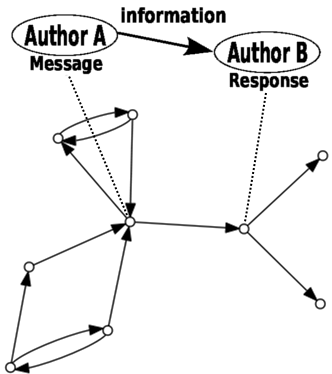
\includegraphics[width=0.5\textwidth]{figs/criaRede3_}
\caption{The formation of interaction networks from exchanged messages. Each node represents a participant. A reply from author B to a message from author A is regarded as evidence that B received information from A and yields a directed edge. Multiple messages add ``weight'' to a directed edge. Further information is provided in Section~\ref{intNet}.}
\label{formationNetwork}
\end{figure}


\subsection{Topological measures}\label{smes}
The derivation of the sectors, described in next subsections,
rely only on the very basic measures of degree and strength.
In order to avoid unnecessary elaborations, the correlation and principal component analysis
were only performed using degree, strength as clustering coefficient.
These measures are defined as follows:
\begin{itemize}
\item Degree $k_i$: number of edges linked to vertex $i$.
\item Strength $s_i$: sum of weights of all edges linked to vertex $i$.
\item Clustering coefficient $cc_i$:
  fraction of pairs of neighbors of $i$ that are linked, i.e. the standard clustering coefficient metric for undirected graphs.
\end{itemize}

\subsection{Sectioning of a network into hub, intermediary and peripheral nodes (Erdös sectioning)}\label{ssec}\label{sectioning}
It is often useful to think of vertices as hubs, peripheral and intermediary.
Authors have therefore derived the peripheral, intermediary and hub sectors of an empirical network
from the comparison against an Erd\"os-R\'enyi network with the same number of edges and vertices,
as depicted in Figure~\ref{fig:setores}. We refer to this procedure as \emph{Erd\"os sectioning},
with the resulting sectors being named as \emph{Erd\"os sectors}.
The degree distribution $\widetilde{P}(k)$ of a real network with a scale-free profile
$\mathcal{N}_f(N,z)$ with $N$ vertices and $z$ edges has less
average degree nodes than the distribution $P(k)$ of an Erd\"os-R\'enyi
network with the same number of vertices and edges.
Indeed, we define in this work the intermediary sector of a network to be the
set of all the nodes whose degree is less abundant in the real network than on the Erd\"os-R\'enyi model:

\begin{equation}\label{criterio}
\widetilde{P}(k)<P(k) \Rightarrow \text{k is intermediary degree}
\end{equation}

If $\mathcal{N}_f(N,z)$ is directed and has no self-loops, the probability of the existence
of an edge between two arbitrary vertices is $p_e=\frac{z}{N(N-1)}$.
A vertex in the ideal Erd\"os-R\'enyi digraph with the same number of vertices and edges,
and thus the same probability $p_e$ for the presence of an edge, will have degree $k$ with probability

\begin{equation}
P(k)=\binom{2(N-1)}{k}p_e^k(1-p_e)^{2(N-1)-k}
\end{equation}

The lower degree fat tail corresponds to the border vertices,
i.e. the peripheral sector or periphery where $\widetilde{P}(k)>P(k)$ and $k$
is lower than any value of $k$ in the intermediary sector.
The higher degree fat tail is the hubs sector,
i.e. $\widetilde{P}(k)>P(k)$ and $k$ is higher than any value of $k$ in the intermediary sector.
The reasoning for this classification is as follows:
vertices so connected that they are virtually nonexistent in the Erd\"os-R\'enyi model, are coherently associated to the hubs sector.
Vertices with very few connections, which are way more abundant than expected in the Erd\"os-R\'enyi model,
are assigned to the periphery.
Vertices with degree values predicted as the most abundant in the Erd\"os-R\'enyi model,
near the average, and less frequent in the real network, are classified as intermediary.
The definition of the Erdös sectors is illustrated in Figure~\ref{fig:setores}.
Further elaboration of the method, such as the usage of in or out-degree,
the consideration of node strength instead of degree,
and derivation of the sectors by using multiple degree and strength measures, are described in~\cite{stab}.
Such developments are omitted in this paper because they are not relevant to the results described here.
In fact, all sectors in this article were obtained by using degree,
but results hold for sectors obtained using the strength.

\clearpage
\begin{figure}[!h]
\centering
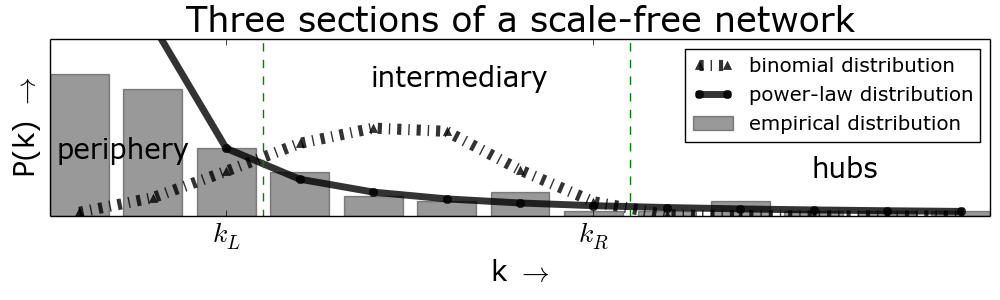
\includegraphics[width=\textwidth]{figs/fser__}
\caption{Classification of vertices by comparing degree
distributions~\cite{stab}.
The binomial distribution of the Erd\"os-R\'enyi network model exhibits more intermediary vertices, while a scale-free network, associated with the power-law distribution, has more peripheral and hub vertices. The sector borders are defined with respect to the intersections of the distributions. Characteristic degrees are in the compact intervals: $[0,k_L]$, $(k_L,k_R]$, $(k_R,k_{max}]$ for the peripheral, intermediary and hubs sectors: the ``Erd\"os sectors''.
Accordingly, the connectivity distribution of empirical interaction networks, e.g. derived from email lists, can be sectioned by comparison against the associated binomial distribution with the same number of vertices and edges. In this figure, a snapshot of 1000 messages from the CPP list yields the degree distribution of an interaction network of 98 nodes and 235 edges. A thorough explanation of the method is provided in Section~\ref{sectioning}.}
\label{fig:setores}
\end{figure}

\subsection{Text-related measures}
This work focuses on simple measurements derived from texts as they have been sufficient for current interests.
The measures are:
\begin{itemize}
\item Frequency of characters: letters, vowels, punctuations and uppercase letters.
\item Number of tokens, frequency of punctuations among tokens, frequency of known words, frequency of words that have Wordnet synsets, frequency of tokens that are stopwords.
\item Mean and standard deviation for word, token sentence and message sizes.
\item Fraction of morphosyntactic classes, such as adverbs, adjectives, nouns and other POS (Part-Of-Speech) tags.
	We implemented a Brill POS tagger because of the massive amount of textual data that we had to analyze (the Brill tagger is very fast).
	We used the ``universal'' tagset described in~\cite{petrov} (developed to account for many languages) and trained the tagger with both Brown and Treebank corpus\footnote{We
		used the full Brown corpus while only 5\% of the Penn Treebank (as included in NLTK~\cite{trabNLTK}).}
	divided into 80/20\% of sentences for training and evaluation. The tagger achieved $94.95\%$ of accuracy.
\item Fraction of words in each Wordnet~\cite{wordnet} top-most hypernyms,
such as abstraction and physical entities for nouns or act for verbs.
\item Mean and standard deviation of the number of Wordnet synset relations, such as holonyms and meronyms, domains, lemmas and verb groups.
\end{itemize}

This selection of measures is based on: 1) the lack of such information in the literature, to the best of our knowledge; 
2) potential relations of these incidences with topological aspects, such as connectivity;
3) the interdependence of textual artifacts suggests that simple metrics should mirror complex and more subtle aspects.
A preliminary study, with the complete works from the Brazilian writer Machado de Assis~\cite{machado},
made clear that the measurements vary with respect to style.

\subsubsection{About Wordnet}
We made use of the statistics derived from the incidence of synsets from the caninical Wordnet~\cite{wordnet} and their characteristics.
This calls for a brief description of what Wordnet is, what is a synset and what are such characteristics:
\begin{itemize}
\item Wordnet groups synonyms into synsets, provides a number of relations among the synsets, definitions and use examples.
\item A ``synset'' is defined by Wordnet documentation as a set of one or more synonyms that are (somewhat) interchangeable without changing the truth value of the proposition in which they occur.
\item Synset characteristics: a synset is associated to other synsets by a number of semantic relations which differ with the POS tag attributed to them.
Examples of such relations include hyponyms and hypernyms (respectively less and more general terms), meronyms and holonyms (respectively ``is part of'' and ``has part''), lemmas (canonical forms of a word), similar words by semantic criteria, entailments.
Some characteristics are derived from the synset in relation to the whole Wordnet network.
In this respect, we used only the maximum and minimum depth of the synset, which are respectively the maximum and minimum number of hypernyms from the synset to the root synset (e.g. 'thing' for nouns).
\end{itemize}

\subsubsection{Relating text and topology}\label{sec:ks}
The topological and textual measures were related by:
\begin{enumerate}
\item textual measures in each of the Erdös sectors, which are delimited by topological criteria as described in Section~\ref{sectioning}.
\item Correlation of metrics of each vertex, facilitating pattern detection involving topology of interaction and language.
\item Principal components formation derived from the usual Principal Component Analysis.
\end{enumerate}

\subsection{Statistical distances}\label{sstat}
An adaptation of the Kolmogorov-Smirnov test~\cite{kolm} was used to observe differences in textual content, as follows.
Let $F$ and $F'$ be two empirical distribution functions, where $n$ and $n'$ are the number of observations on each sample.
The two-sample Kolmogorov-Smirnov test rejects the null hypothesis, that the samples are drawn from the same underlying distribution, if:
\begin{equation}\label{eq:ks}
D_{F,F'} > c(\alpha)\sqrt{\frac{n+n'}{nn'}}
\end{equation}

\begin{figure}[!htbp] %h or !htbp
\vspace{-2pt}
\begin{center}
	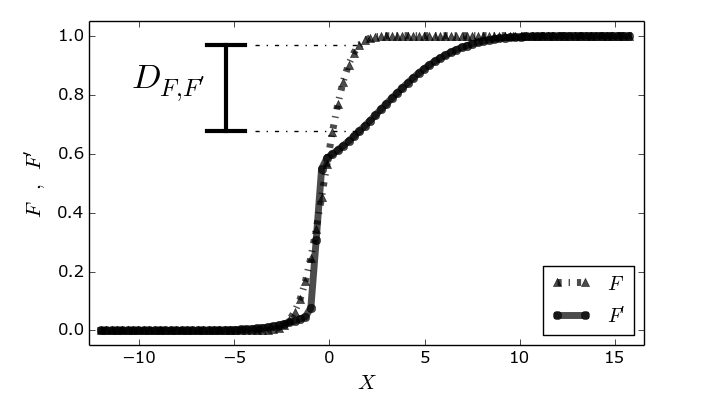
\includegraphics[width=0.64\textwidth]{./figs/Dnn}
	\caption{The Kolmogorov-Smirnov statistic $D_{F,F'}$: the maximum difference between
		two cumulative distribution functions.}
	\label{fig:dnn}
\end{center}
\end{figure}


\noindent where $D_{F,F'}=sup_x[F - F']$ is the Kolmogorov-Smirnov statistic
(illustrated in Figure~\ref{fig:dnn})
and $c(\alpha)$ is related to the significance level $\alpha$ by:

\begin{table}[H]
\centering
\begin{tabular}{l|c c c c c c}
$\alpha$ & 0.1 & 0.05 & 0.025 & 0.01 & 0.005 & 0.001 \\
$c(\alpha)$ & 1.22 & 1.36 & 1.48 & 1.63 & 1.73 & 1.95 \\
\end{tabular}
\end{table}

In comparing two empirical distribution functions,
$D_{F,F'}$ is given, as are $n$ and $n'$.
All terms in equation~\ref{eq:ks} are positive and $c(\alpha)$ can be isolated:

\begin{equation}\label{eq:ks2}
c(\alpha) < \frac{D_{F,F'}}{\sqrt{\frac{n+n'}{nn'}}} = c'
\end{equation}

When $c'$ is high, corresponding low values of $\alpha$ favor rejecting the null hypothesis.
For example, when $c'$ is greater than $\approx 1.7$, one might assume that $F$ and $F'$ differ.
We used $c'$ as a measure of how much
the distributions differ
and for deriving hypotheses
about how different are the underlying mechanisms of generation of texts.
In~\cite{kolm},
systematic measurements of the $c'$ statistic
illustrate that $c'$ and $D_{F,F'}$ are consistent and useful in considering the
similarity or difference in the distributions underlying sets of observations.
A note of caution should be given here: what is a difference in distributions
might vary with context.
A $D_{F,F'}$ of only $0.0001$ will yield a very large $c'$ if $n$ and $n'$ are large enough.
On the other hand, a large $D_{F,F'}$ with a small $c'$ is not a strong evidence that
the distributions differ.
Therefore, we consider both $D_{F,F'}$ and $c'$ simultaneously in our analysis.
Each text-related measure yields a histogram for the whole network, and one for each
of the Erdös sectors.
To obtain the histograms, one value was obtained through each message.

\section{Results and discussion}\label{sres}\label{sec:tresults}
The consideration of all measures and all distances results in a vast number of measurements, comparisons and tables.
Also, a thorough discussion of these outcomes becomes lengthy and tiresome.
We here present a summary of the findings and
a more comprehensive presentation is available at~\cite{thesis} if
the reader finds necessary.
Furthermore, we recall that the Supplementary document of this paper provides all measurements in all 18 randomly selected email lists.
Also in the Supplementary document, we relate the email lists to each numerical
TAG in the tables of the following sections.

The most important result is the strong statistical evidence of differentiation of each Erd\"os sector with respect to the language used.
This conclusion can be reached by observing the differences in the measurements of textual features in
each sector, and is supported on firm theoretical grounds by using the adapted Kolmogorov-Smirnov test presented in Section~\ref{sec:ks}.
% derived from the kolmogorov-smirnov test adaptation
Other relevant results are:
\begin{itemize}
\item the identification of patterns in the frequency of use of nouns, adverbs, sizes of words, depth of Wordnet synsets and other linguistic features, in the network as a whole.
  We did not find in the literature any indication for such values, thus we understand useful to report e.g. that about 15\% of the characters are spaces and that nouns often account for more than 25\% of the words.
These values are available in the Supplementary document and not in the body of this paper,
since the focus here is the evidence that texts from distinct sectors differ.
\item Evidence of what is different in the language used by each Erd\"os sector. For example: hubs were found to use more contractions,
more common words, and less punctuation if compared to the rest of the network,
especially the peripheral sector.
In general, the rise or fall of a text-related metric is not relevant or is monotonic along connectivity,
but some of them reach extreme values in the intermediary sector.
\end{itemize}

The next sections summarize results of immediate interest
and further insights can be obtained by skimming through
the tables of the Supplementary document of this paper.
We illustrate with just one table of each kind,
and from networks obtained with 2000 messages.
After analysing the networks in many scales,
we considered the networks obtained by constructed using 1000 and 2000 messages as representative for the phenomena being characterized.
The findings with 1000 messages are the same as with 2000 messages.
This motivated the exclusion of the tables with measurements in
networks of 1000 messages.

\subsection{General characteristics of activity distribution among sectors}\label{sec:gen}
In order to support a relevant consideration of findings derived from text-related measurements,
this section provides a glance at the general structure of these networks,
with emphasis on the activity of the Erdös sectors.
In almost all our observations,
the peripheral sector was responsible for starting most of the discussion threads,
i.e. for sending messages to the list which are not replies.
This is surprising since the peripheral sector is responsible for fewer messages.
It suggests a complementarity between peripheral diversity and hub specialization, which, on its turn, emphasizes the understanding of the interaction network as a meaningful system. 
These assertions are condensed in Table~\ref{geralListas}.
Less often, the intermediary sector is responsible for the largest number of messages and of threads.
Also meaningful is that the hubs sector is responsible for most of the messages, which is not obvious: hub participants are far more active but way less numerous. Interestingly, in such a setting where every characteristic differs with respect to
distinct sectors, there was no evidence of difference on the size of the threads started by each sector.
\begin{table}[h!]
\begin{center}
\begin{tabular}{| l || c | c | c | c |}\hline
 & {\bf g.} & {\bf p.} & {\bf i.} & {\bf h.} \\\hline\hline
$N$ & 17.00  & 7.00  & 6.00  & 4.00 \\
$N_{\%}$ & 100.00  & 41.18  & 35.29  & 23.53 \\\hline
$M$ & 100.00  & 11.00  & 37.00  & 52.00 \\
$M_{\%}$ & 100.00  & 11.00  & 37.00  & 52.00 \\\hline
$\Gamma$ & 18.00  & 4.00  & 8.00  & 6.00 \\
$\Gamma_{\%}$ & 100.00  & 22.22  & 44.44  & 33.33 \\\hline
$\frac{\Gamma}{M}\%$ & 18.00  & 36.36  & 21.62  & 11.54 \\
$\mu(\gamma)$ & 2.67  & 2.50  & 2.75  & 2.67 \\
$\sigma(\gamma)$ & 0.47  & 0.50  & 0.43  & 0.47 \\\hline
\end{tabular}
\caption{Distribution of participants, messages and threads among each Erd\"os sector ({\bf p.} for periphery, {\bf i.} for intermediary, 
    {\bf h.} for hubs) in a total time period of 0.71 years (from 2007-04-24T18:54:28 to 2008-01-10T19:17:26). $N$ is the number of participants, $M$ is the number of messages, $\Gamma$ is the number of threads, and $\gamma$ is the number of messages in a thread.
    The \% denotes the usual `per cent' with respecto to the total quantity ($100\%$ for {\bf g.})
    while $\mu$ and $\sigma$ denote mean and standard deviation.}
\end{center}
\end{table}

\subsection{Evidence that the texts from Erd\"os sectors differ}\label{subsec:di}
This is the most important outcome from this paper: there strong enough evidence
to support the assertion that the language used by distinct Erd\"os sectors are different.
Figure~\ref{fdif} illustrates, and Tables~\ref{tab:kolTok}-\ref{tab:kolPctInter}
exemplify three results:
\begin{itemize}
 \item The statistical evidence that the textual production of the Erd\"os sectors is different.
	 This can be noticed from the high values of $c'$ on these tables, clearly above reference values used for the acceptance of the null hypothesis (the null hypothesis being that the probability distributions generating the samples are the same). Also, we regarded as non-negligible the values often above 0.1 for the Kolmogorov-Smirnov statistics (the maximum difference between the cumulative distributions), which we recognized as relevant for assuming differences in the underlying distributions in our study (see Section~\ref{sec:ks}).
  \item Intermediary sectors sometimes exhibit greater differences 
against the periphery and hubs than these extreme sectors between themselves 
(Tables~\ref{tab:kolTok} and~\ref{tab:kolSub}).
This differentiation of the three sectors is a further indicative that the Erd\"os Sectioning described in Section~\ref{sectioning} reveals meaningful sectors of the networks.
 \item The evidence of difference (as measured by $c'$) between sectors on the same network (Tables~\ref{tab:kolTok}-\ref{tab:kolPct}) is often larger than found between the same sector from distinct networks (Tables~\ref{tab:kolSubInter}-\ref{tab:kolPctInter}).
 \end{itemize}

\begin{figure}[!h]
\centering
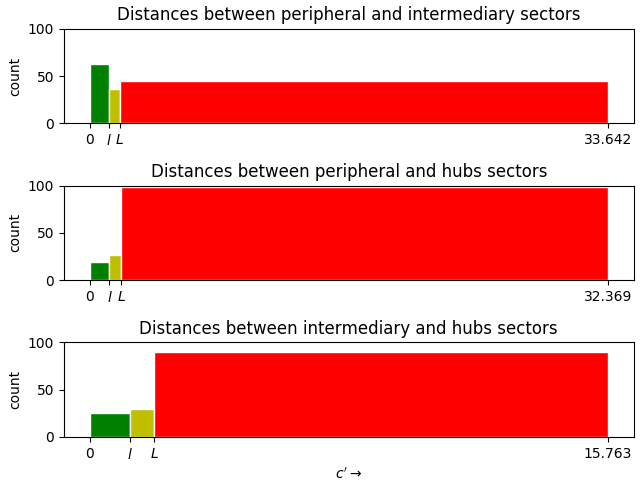
\includegraphics[width=0.9\textwidth]{figs/hists}
  \caption{Histograms of the $c'$ statistic between the Erd\"os sectos for all the language-related measurements performed. The histogram bins are limited by the values $l=1.22$, and $L=1.95$, which are related to the significance levels of 0.1 and 0.001, respectively, as described in Section~\ref{sstat}. 
  In qualitative terms, one may associate the bars to:
  measurements that are not evidence of difference (blue),
  measurements that are evidence of difference (green),
  and measurements that are strong evidence of difference (red).
  Notice that, although the $c'$ values obtained by comparing the peripheral and intermediary sectors present less values in the red bar, the values reach the magnitudes comparable to the highest values obtained by comparing the peripheral and hubs sectors.
  Further information is provided in Section~\ref{subsec:di}.}
\label{fdif}
\end{figure}

Two measurements for each pair of sectors are in Tables~\ref{tab:kolTok}-\ref{tab:kolPct}.
 The top value is $c'$ while the bottom value is the Kolmogorov-Smirnov statistic.
 In Tables~\ref{tab:kolSubInter}-\ref{tab:kolPctInter} only $c'$ values are shown to illustrate
 that the measurements found between networks are comparable to (and often lower than) measurements found between sectors of a same network.
 \begin{table}[h!]
\begin{center}
	\caption{Measurements of $c'$ and the KS statistic related to sizes of tokens between the Erd\"os sectors and the whole network. The abbreviations are: g for global, p for peripheral, i for intermediary, h for hubs. See Section~\ref{sec:ks} for and explanation of the measures and Section~\ref{subsec:di} for discussion. TAG of list: 6}
\label{tab:kolTok}
\begin{tabular}{l ? c c c | c c c}
{\bf } & {\bf p-g} & {\bf i-g} & {\bf h-g} & {\bf p-i} & {\bf p-h} & {\bf i-h} \\\hline
$c'$ & 4.327  & 17.168  & 7.851  & 18.907  & 7.833  & 15.540 \\
KS & 0.014  & 0.115  & 0.044  & 0.129  & 0.045  & 0.129 \\
\end{tabular}
\end{center}
\end{table}

 \begin{table}[h!]
\begin{center}
\caption{Measurements of $c'$ and the KS statistic related to sizes of known words between the Erd\"os sectors and the whole network. The abbreviations are: g for global, p for peripheral, i for intermediary, h for hubs. See Section~\ref{sec:ks} for and explanation of the measures and Section~\ref{subsec:di} for discussion. TAG of list: 1}
\begin{tabular}{l | c c c c c c}
{\bf } & {\bf p-g} & {\bf i-g} & {\bf h-g} & {\bf p-i} & {\bf p-h} & {\bf i-h} \\\hline
$c'$ & 5.904  & 5.264  & 5.549  & 9.547  & 7.073  & 4.058 \\
KS & 0.043  & 0.040  & 0.150  & 0.083  & 0.193  & 0.111 \\
\end{tabular}
\end{center}
\end{table}

 \begin{table}[h!]
\begin{center}
\caption{Measurements of $c'$ and the KS statistic related to sizes of sentences between the Erd\"os sectors and the whole network. The abbreviations are: g for global, p for peripheral, i for intermediary, h for hubs. See Section~\ref{sec:ks} for and explanation of the measures and Section~\ref{subsec:di} for discussion. TAG of list: 2}
\begin{tabular}{l ? c c c | c c c}
{\bf } & {\bf p-g} & {\bf i-g} & {\bf h-g} & {\bf p-i} & {\bf p-h} & {\bf i-h} \\\hline
$c'$ & 0.733  & 2.077  & 2.834  & 1.642  & 2.589  & 4.139 \\
KS & 0.020  & 0.038  & 0.059  & 0.048  & 0.080  & 0.097 \\
\end{tabular}
\end{center}
\end{table}


 \begin{table}[h!]
\begin{center}
\caption{Measurements of $c'$ and the KS statistic related to the frequency of use of adjectives between the Erd\"os sectors and the whole network. The abbreviations are: g for global, p for peripheral, i for intermediary, h for hubs. See Section~\ref{sec:ks} for and explanation of the measures and Section~\ref{subsec:di} for discussion. TAG of list: 3}
\begin{tabular}{l ? c c c | c c c}
{\bf } & {\bf p-g} & {\bf i-g} & {\bf h-g} & {\bf p-i} & {\bf p-h} & {\bf i-h} \\\hline
$c'$ & 0.461  & 0.564  & 0.617  & 0.385  & 0.800  & 0.986 \\
KS & 0.011  & 0.010  & 0.010  & 0.011  & 0.021  & 0.020 \\
\end{tabular}
\end{center}
\end{table}

 \begin{table}[h!]
\begin{center}
\caption{Measurements of $c'$ and the KS statistic related to the frequency of use of nouns between the Erd\"os sectors and the whole network. The abbreviations are: g for global, p for peripheral, i for intermediary, h for hubs. See Section~\ref{sec:ks} for and explanation of the measures and Section~\ref{subsec:di} for discussion. TAG of list: 1}\label{tab:kolSub}
\begin{tabular}{l | c c c c c c}
{\bf } & {\bf p-g} & {\bf i-g} & {\bf h-g} & {\bf p-i} & {\bf p-h} & {\bf i-h} \\\hline
$c'$ & 0.642  & 1.791  & 6.936  & 1.007  & 6.970  & 7.510 \\
KS & 0.023  & 0.067  & 0.537  & 0.044  & 0.560  & 0.607 \\
\end{tabular}
\end{center}
\end{table}

 \begin{table}[h!]
\begin{center}
	\caption{Measurements of $c'$ and the KS statistic related to the frequency of use of punctuations between the Erd\"os sectors and the whole network. The abbreviations are: g for global, p for peripheral, i for intermediary, h for hubs. See Section~\ref{sec:ks} for and explanation of the measures and Section~\ref{subsec:di} for discussion. TAG of list: 8}\label{tab:kolPct}
\begin{tabular}{l | c c c c c c}
{\bf } & {\bf p-g} & {\bf i-g} & {\bf h-g} & {\bf p-i} & {\bf p-h} & {\bf i-h} \\\hline
$c'$ & 1.380  & 3.583  & 2.894  & 1.718  & 2.871  & 5.398 \\
KS & 0.039  & 0.069  & 0.046  & 0.054  & 0.085  & 0.114 \\
\end{tabular}
\end{center}
\end{table}

 \begin{table}
  \centering
  \caption{$c'$ values for the frequency of use of nouns. Comparison of the same sector between lists, each author is an observation. See subsection~\ref{subsec:di} for discussion and directions.}
    \small
\setlength{\tabcolsep}{.06667em}
  \begin{tabular}{l|| c|c|c|c|c|c}\hline
& CPP-LAD & CPP-LAU & CPP-ELE & LAD-LAU & LAD-ELE & LAU-ELE \\\hline\hline
P & 1.35 & 4.05 & 5.80 & 3.00 & 5.41 & 4.94 \\\hline
I & 1.27 & 0.78 & 4.01 & 0.84 & 3.84 & 3.94 \\\hline
H & 0.98 & 1.94 & 3.17 & 1.32 & 3.82 & 4.47 \\\hline
  \end{tabular}
\begin{flushleft}\footnotesize
		Source: By the author.\
\end{flushleft}
  \label{tab:kolSubInter}
\end{table}

\begin{table}
  \centering
  \caption{$c'$ values for the frequency of use of adjectives. Comparison of the same sector between lists, each author is an observation. See subsection~\ref{subsec:di} for discussion and directions.}
    \small
\setlength{\tabcolsep}{.06667em}
  \begin{tabular}{l|| c|c|c|c|c|c}\hline
 & CPP-LAD & CPP-LAU & CPP-ELE & LAD-LAU & LAD-ELE & LAU-ELE \\\hline\hline
P & 0.44 & 0.34 & 2.57 & 0.20 & 2.32 & 2.37 \\\hline
I & 0.74 & 0.99 & 3.72 & 0.32 & 3.37 & 3.10 \\\hline
H & 0.26 & 0.32 & 3.72 & 0.29 & 4.36 & 4.24 \\\hline
  \end{tabular}
\begin{flushleft}\footnotesize
		Source: By the author.\
\end{flushleft}
  \label{tab:kolAdjInter}
\end{table}

\begin{table}
  \centering
  \caption{$c'$ values for the frequency of use stopwords. Comparison of the same sector between lists, each author is an observation. See subsection~\ref{subsec:di} for discussion and directions.}
    \small
\setlength{\tabcolsep}{.06667em}
  \begin{tabular}{l|| c|c|c|c|c|c}\hline
 & CPP-LAD & CPP-LAU & CPP-ELE & LAD-LAU & LAD-ELE & LAU-ELE \\\hline\hline
P & 3.31 & 3.26 & 6.68 & 0.57 & 5.36 & 5.41 \\\hline
I & 1.45 & 1.08 & 5.16 & 0.91 & 5.00 & 4.92 \\\hline
H & 0.98 & 0.68 & 4.35 & 1.05 & 4.73 & 5.01 \\\hline
  \end{tabular}
\begin{flushleft}\footnotesize
		Source: By the author.\
\end{flushleft}
  \label{tab:kolSwInter}
\end{table}

\begin{table}
  \centering
  \caption{$c'$ values for the frequency of use of punctuations among characters. Comparison of the same sector between lists, each author is an observation. See subsection~\ref{subsec:di} for discussion and directions.}
    \small
\setlength{\tabcolsep}{.06667em}
  \begin{tabular}{l|| c|c|c|c|c|c}\hline
 & CPP-LAD & CPP-LAU & CPP-ELE & LAD-LAU & LAD-ELE & LAU-ELE \\\hline\hline
P & 5.74 & 4.88 & 8.28 & 2.23 & 5.37 & 6.60 \\\hline
I & 3.23 & 2.49 & 4.16 & 0.96 & 3.40 & 3.51 \\\hline
H & 2.49 & 1.87 & 4.02 & 1.36 & 3.05 & 3.71 \\\hline
  \end{tabular}
\begin{flushleft}\footnotesize
		Source: By the author.\
\end{flushleft}
  \label{tab:kolPctInter}
\end{table}
 


\subsection{What differs and how the texts from the sectors differ}
 In the next sections we will look through language-related measurements
 and summarize the findings about what might be different in
 the textual features of the sectors.
 One should keep in mind that our core result is the evidence that
 the texts from distinct sectors differ.
 The following discussion of what differs and how it differs
 is interesting but is both derived from less strong statistical evidence and less crucial for our current stage of researching these structures.
 Nonetheless, for the sake of clarity, we state the main findings in this respect:
 \begin{itemize}
\item Peripherals were found to use more nouns while hubs use more verbs and adverbs. The fraction of adjectives did not change as irrefutably with respect to connectivity, but given that nouns are more numerous in the periphery sector, there are more adjectives per noun in the hubs sector texts.
\item Sentences and messages were found smaller in the more connected sectors although punctuation was more incident in the less connected sectors.
\item The differences found in analyzing Wordnet synset hypernyms were found less well behaved. Often, the sectors exhibit noticeable differences but greater and smaller incidences are found in all sectors (but in different networks). Some of these incidences are more systematic and this analysis assisted by Wordnet is the only semantic analysis we made, which is why we included these results.
\end{itemize}

Appendix~\ref{ap:textd} presents tables with counts for larger incidence in each sector throughout the networks. In the following discussion we provide example tables for each set of measurements.
In the measurements derived from synset hypernyms the example tables were less meaningful because of the greater variability and therefore we present the counts of greater incidence directly.
In any case, the measurements for each of the networks are in the Supplementary document of this paper.
The analysis of the measurements
is not trivial because of the number of different measures
and because differences in measurements are not obviously relevant.
Furthermore, there is too much variation among networks
which renders worthless the usual global measurements such as mean and variance when obtained from all the systems at once.
In order to obtain consistent results, we considered \emph{weak evidence of difference} in sectors in a network
if maximum measure is at least 10\% greater than minimum measure,
i.e. $\frac{maximum\;measure}{minumum\;measure}>1.1$.
We considered \emph{evidence of difference} in sectors in a network if
$\frac{maximum\;measure}{minumum\;measure}>1.2$.
When 
$\frac{maximum\;measure}{minumum\;measure}>1.5$, we considered \emph{strong evidence of difference}.
We then looked through each measure in all networks to reach compelling observations about the
differences of sectors through all networks.
Instead of the counts of maximum incidences, we also performed a weighted count:
when the evidence was weak, the sector received an add of $0.5$ in the weighted count;
then the evidence was strong, the sector received an add of $2$ in the weighted count.
The results were qualitatively the same, so we omit the tables with weighted counts.
Also useful here is the definition of lower sectors (peripheral and intermediary),
upper sectors (intermediary and hubs) and extreme sectors (peripheral and hubs).
We should also state when measurements peak often at the intermediary sector,
be it a maximum or minimum peak.

The tables that follow have terms for measurements that might be immediately inferred,
but this depends on the background of the reader.
Therefore the terms are explicitly defined in Appendix~\ref{ap:msTerms}.

\subsection{Characters}\label{sec:cha}
Most often, peripheral and intermediary sectors use more digits, uppercase letters and punctuation.
Hubs sectors were found to use more spaces in most cases. 
These results are illustrated in Table~\ref{tab:cha}.
\begin{table}[h!]
\begin{center}
\begin{tabular}{| l || c | c | c | c |}\hline
 & {\bf g.} & {\bf p.} & {\bf i.} & {\bf h.} \\\hline\hline
$chars$ & 82933  & 7162  & 28170  & 47601 \\
$chars_{\%}$ & 100.00  & 8.64  & 33.97  & 57.40 \\\hline
$\frac{spaces}{chars}$ & 14.96  & 13.59  & 15.21  & 15.01 \\
$\frac{punct}{chars-spaces}$ & 8.17  & 6.98  & 8.03  & 8.44 \\
$\frac{digits}{chars-spaces}$ & 0.90  & 1.97  & 0.77  & 0.80 \\\hline
$\frac{letters}{chars-spaces}$ & 88.72  & 88.88  & 88.98  & 88.54 \\
$\frac{vogals}{letters}$ & 40.47  & 39.17  & 40.72  & 40.53 \\
$\frac{uppercase}{letters}$ & 5.27  & 6.22  & 5.39  & 5.05 \\\hline
\end{tabular}
\caption{Characters in each Erd\"os sector ({{\bf p.}} for periphery, {{\bf i.}} for intermediary, 
    {{\bf h.}} for hubs).}
\end{center}
\end{table}
\FloatBarrier

\subsection{Tokens and words}\label{subsec:tw}
Hubs were found to use more contractions and stopwords, while the peripheral sectors exhibit a greater incidence of punctuations among tokens.
Although the token diversity ($\frac{|tokens \neq|}{|tokens|}$) found in the peripheral sector is greater,
this result has the masking artifact that the peripheral sector corpus is smaller, yielding a larger token diversity.
This can be noticed by the token diversity of the whole network, which is lower than in any of the sectors.
These results are exemplified in Table~\ref{tab:tokensInline}
where mean and variance were taken with respect to the length in characters of tokens, known words and stopwords.
\begin{table}[h!]
\begin{center}
\begin{tabular}{| l || c | c | c | c |}\hline
 & {\bf g.} & {\bf p.} & {\bf i.} & {\bf h.} \\\hline\hline
$tokens$ & 17964  & 1539  & 6064  & 10361 \\
$tokens_{\%}$ & 100.00  & 8.57  & 33.76  & 57.68 \\
$tokens \neq$ & 15.21  & 32.16  & 25.89  & 18.02 \\\hline
$\frac{knownw}{tokens}$ & 36.48  & 35.74  & 38.03  & 35.69 \\
$\frac{knownw \neq}{knownw}$ & 8.62  & 24.73  & 15.31  & 10.84 \\\hline
$\frac{stopw}{knownw}$ & 11.43  & 10.00  & 11.71  & 11.47 \\
$\frac{punct}{tokens}$ & 23.73  & 22.35  & 22.82  & 24.47 \\
$\frac{contrac}{tokens}$ & 0.01  & 0.00  & 0.00  & 0.02 \\\hline\hline
$\mu(\overline{tokens})$ & 3.84  & 3.94  & 3.86  & 3.82 \\
$\sigma(\overline{tokens})$ & 2.99  & 3.10  & 2.96  & 2.99 \\\hline
$\mu(\overline{knownw})$ & 3.28  & 3.27  & 3.32  & 3.26 \\
$\sigma(\overline{knownw})$ & 1.81  & 1.86  & 1.80  & 1.81 \\\hline
$\mu(\overline{knownw \neq})$ & 5.12  & 4.35  & 4.92  & 4.98 \\
$\sigma(\overline{knownw \neq})$ & 2.20  & 2.22  & 2.25  & 2.15 \\\hline
$\mu(\overline{stopw})$ & 1.77  & 1.84  & 1.77  & 1.76 \\
$\sigma(\overline{stopw})$ & 0.74  & 0.76  & 0.73  & 0.75 \\\hline
\end{tabular}
\caption{Token sizes in each Erd\"os sector ({{\bf p.}} for periphery, {{\bf i.}} for intermediary, {{\bf h.}} for hubs).}
\end{center}
\end{table}
\FloatBarrier

\subsection{Sizes of sentences}\label{subsec:ss}
Hubs present the lowest average sentence size
in terms of characters, tokens, known words or punctuations.
This result is illustrated in Table~\ref{tab:sizesSents}
and might be considered counterintuitive given that punctuation
is more abundant in the texts of less connected participants.
\begin{table}[h!]
\begin{center}
\begin{tabular}{| l || c | c | c | c |}\hline
 & {\bf g.} & {\bf p.} & {\bf i.} & {\bf h.} \\\hline\hline
$sents$ & 558  & 45  & 211  & 304 \\
$sents_{\%}$ & 99.64  & 8.04  & 37.68  & 54.29 \\\hline
$\mu_S(chars)$ & 147.51  & 158.07  & 132.44  & 155.44 \\
$\sigma_S(chars)$ & 147.95  & 154.11  & 135.56  & 154.01 \\\hline
$\mu_S(tokens)$ & 32.21  & 34.22  & 28.75  & 34.09 \\
$\sigma_S(tokens)$ & 32.08  & 32.64  & 29.17  & 33.60 \\\hline
$\mu_S(knownw)$ & 9.90  & 9.82  & 9.10  & 10.39 \\
$\sigma_S(knownw)$ & 10.37  & 11.34  & 9.14  & 10.92 \\\hline
$\mu_S(stopw)$ & 1.18  & 1.11  & 1.15  & 1.20 \\
$\sigma_S(stopw)$ & 1.57  & 1.22  & 1.52  & 1.64 \\\hline
$\mu_S(puncts)$ & 7.65  & 7.67  & 6.57  & 8.35 \\
$\sigma_S(puncts)$ & 11.30  & 8.19  & 10.69  & 11.98 \\\hline
\end{tabular}
\caption{Sentences sizes in each Erd\"os sector ({{\bf p.}} for periphery, {{\bf i.}} for intermediary, {{\bf h.}} for hubs).}
\end{center}
\end{table}
\FloatBarrier

\subsection{Messages}\label{subsec:mm}
Connectivity was found correlated to smaller messages in terms of characters, tokens, known words and punctuations.
Connectivity was also found correlated to smaller messages in terms of the number of sentences, but
it was less consistent.
Interestingly, the number of stopwords per message was found greater in all sectors (but in different networks).
This result is exemplified in Table~\ref{tab:sizesMsgs}.
\begin{table}[h!]
\begin{center}
\begin{tabular}{| l || c | c | c | c |}\hline
 & {\bf g.} & {\bf p.} & {\bf i.} & {\bf h.} \\\hline\hline
$msgs$ & 100  & 11  & 37  & 52 \\
$msgs_{\%}$ & 100.00  & 11.00  & 37.00  & 52.00 \\\hline
$\mu_M(sents)$ & 6.54  & 4.91  & 6.62  & 6.83 \\
$\sigma_M(sents)$ & 5.09  & 3.26  & 6.28  & 4.35 \\\hline
$\mu_M(tokens)$ & 179.79  & 140.00  & 163.97  & 199.46 \\
$\sigma_M(tokens)$ & 183.42  & 71.56  & 182.94  & 197.24 \\\hline
$\mu_M(knownw)$ & 55.24  & 40.18  & 51.92  & 60.79 \\
$\sigma_M(knownw)$ & 61.67  & 26.49  & 59.82  & 67.33 \\\hline
$\mu_M(stopw)$ & 6.55  & 4.55  & 6.54  & 6.98 \\
$\sigma_M(stopw)$ & 6.92  & 3.11  & 7.11  & 7.29 \\\hline
$\mu_M(puncts)$ & 42.77  & 31.36  & 37.46  & 48.96 \\
$\sigma_M(puncts)$ & 48.91  & 14.92  & 48.61  & 52.78 \\\hline
$\mu_M(chars)$ & 829.31  & 651.09  & 761.35  & 915.37 \\
$\sigma_M(chars)$ & 878.54  & 342.18  & 889.47  & 937.65 \\\hline
\end{tabular}
\caption{Messages sizes in each Erd\"os sector ({{\bf p.}} for periphery, {{\bf i.}} for intermediary, {{\bf h.}} for hubs).}
\end{center}
\end{table}
\FloatBarrier

\subsection{POS tags}\label{subsec:pos}
We found that lower connectivity yields more nouns and less verbs and adverbs.
Also, the fraction of adjectives does not change consistently,
but given that peripherals use more nouns,
we can conclude that hubs use more adjectives per noun.
This suggests that the networks gather issues
through the peripheral sector. 
These issues are qualified and proposed to be acted upon
by the more connected participants.
This is a further indicative that peripheral sectors
are related to diversity while hubs relate to specialization.
These results are exemplified in Table~\ref{tab:pos}.
Weaker evidence was found that hubs use more \emph{adpositions},
determinants and 'particles and other functional words' while
peripherals use more numerals.
\begin{table}[h!]
\begin{center}
\begin{tabular}{| l || c | c | c | c |}\hline
 & {\bf g.} & {\bf p.} & {\bf i.} & {\bf h.} \\\hline\hline
NOUN & 56.40  & 58.68  & 55.67  & 56.50 \\
X & 16.46  & 16.20  & 16.58  & 16.42 \\\hline
ADP & 7.22  & 6.78  & 7.38  & 7.18 \\
DET & 6.07  & 5.12  & 6.41  & 6.02 \\\hline
VERB & 5.13  & 4.46  & 5.90  & 4.75 \\\hline
ADJ & 3.29  & 3.97  & 2.87  & 3.44 \\
ADV & 2.07  & 2.15  & 1.82  & 2.21 \\\hline
PRT & 1.79  & 1.32  & 1.51  & 2.04 \\
PRON & 1.18  & 0.83  & 1.48  & 1.04 \\
NUM & 0.33  & 0.50  & 0.27  & 0.34 \\
CONJ & 0.07  & 0.00  & 0.12  & 0.05 \\
PUNC & 0.00  & 0.00  & 0.00  & 0.00 \\\hline
\end{tabular}
\caption{POS tags in each Erd\"os sector ({{\bf p.}} for periphery, {{\bf i.}} for intermediary, {{\bf h.}} for hubs).
    Universal POS tags~\cite{{petrov}}:
    VERB - verbs (all tenses and modes);
    NOUN - nouns (common and proper);
    PRON - pronouns;
    ADJ - adjectives;
    ADV - adverbs;
    ADP - adpositions (prepositions and postpositions);
    CONJ - conjunctions;
    DET - determiners;
    NUM - cardinal numbers;
    PRT - particles or other function words;
    X - other: foreign words, typos, abbreviations;
    PUNCT - punctuation.
}
\end{center}
\end{table}
\FloatBarrier


\subsection{Wordnet-related results}
For correctly analyzing text production in terms of the Wordnet lexical database,
we only considered words that had synsets\footnote{
  Examples of categories of tokens without synsets are stopwords, punctuations, numerals, acronyms and typos.}
and that had at least one synset with the POS tag obtained with the POS tagger.
There are often more than one synset with the same POS tag for each word,
thus we chose the most frequent synset as ranked by Wordnet.
This resulted in portions of tokens considered of $\approx 30\%$,
but of more than $90\%$ of all tokens with Wordnet synsets.
This yields less strong results, but which we found still relevant as no similar outcome was found in the scientific literature by the authors.
Moreover, observations seem consistent and meaningful,
Measures regarding Wordnet synsets often reach an extreme value (maximum or minimum)
in the intermediary sector, which we understood as evidence that:
\begin{itemize}
\item the Erd\"os sectors are in fact relevant for human social structures, at least to the ones analyzed in this thesis.
\item Human social networks present relations between connectivity and semantics.
\item The intermediary sector might hold a deeper identity than that of a sector bounded by hubs and periphery sectors.
\item The analysis of the language employed in social networksm, using Wordnet, reveals aspects of the structures which are not clear though the non-semantic analysis we performed.
\end{itemize}

\subsubsection{Wordnet POS tags}\label{subsec:wnpos}
The observations here are somewhat consistent with those in Section~\ref{subsec:pos}:
peripherals use more nouns and less verbs and adverbs.
The variation is related to adjectives, which was found more frequent in the hubs.
These results are illustrated in Table~\ref{tab:wnpos}.
\begin{table}[h!]
\begin{center}
\begin{tabular}{| l || c | c | c | c |}\hline
 & {\bf g.} & {\bf p.} & {\bf i.} & {\bf h.} \\\hline\hline
N & 88.79  & 91.15  & 87.41  & 89.26 \\\hline
ADJ & 6.11  & 7.08  & 5.34  & 6.42 \\\hline
VERB & 0.24  & 0.00  & 0.38  & 0.19 \\\hline
ADV & 4.86  & 1.77  & 6.86  & 4.13 \\\hline\hline
POS & 21.05  & 22.01  & 21.61  & 20.58 \\\hline
POS! & 72.54  & 74.83  & 71.48  & 72.85 \\\hline
\end{tabular}
\caption{Percentage of synsets with each of the POS tags used by Wordnet. The last lines give the percentage of words considered from all of the tokens (POS) and from the words with synset (POS!). The tokens not considered are punctuations, unrecognized words, words without synsets, stopwords and words for which Wordnet has no synset  tagged with POS tags . Values for each Erd\"os sectors are in the columns {{\bf p.}} for periphery, {{\bf i.}} for intermediary, {{\bf h.}} for hubs.}
\end{center}
\end{table}
\FloatBarrier

\subsubsection{Wordnet synsets characteristics}\label{subsec:wn1}
Wordnet synsets with different POS tags have different relations (to other synsets).
Therefore, we made separate observations about each POS tag.
In each synset we performed a count of the number of the relations (e.g. max depth, hyponyms),
thus yielding a mean and variance of each of the number of relations.
\begin{itemize}
\item Nouns, exemplified in Table~\ref{tab:wnn}.
\begin{itemize}
\item Minimum and maximum depth: 
differences were found in the mean of minimum and maximum depth of a synset between email lists,
but not once among sectors of a network.
Differences between the variance of minimum and maximum depth of synsets of sectors were found mostly nonexistent or weak.
\item Holonyms:
differences in the number of holonyms per word were present in $\approx 85\%$ of the networks and were
more incident in the lower sectors in $\approx 90\%$ of the observations in which we found such differences.
Differences in the variance in the number of holonyms were also found with the same regularity,
but were greater in the upper sectors in $\approx 80\%$ of the networks.
Both mean and variance of the number of holonyms peaked in the intermediary sector in $\approx50\%$ of the observations.
\item Meronyms:
differences in the number of meronyms of nouns were present in $\approx 90\%$ of the networks and were
more incident in the lower sectors in $\approx 80\%$ of the observations in which we found such differences.
Differences in the variance in the number of meronyms were found in $100\%$ of the networks and was often strong.
The variance was greater in the periphery in $66.66\%$ and in the lower sectors in $\approx 90\%$ of the observations.
\item Domain:
differences in the mean and variance of the number of domains of words were found respectively in $90\%$ and $50\%$ of the networks and maximum values were found evenly distributed across sectors.
Peaks were found in the intermediary sector in $\approx 50\%$ of the networks.
\item Lemmas:
differences in the mean and variance of the number of lemmas of words were found respectively in $40\%$ and $55\%$ of the networks.
In $\approx 90\%$ of the cases where there was difference in the mean, the maximum number of lemmas was found in the periphery.
Peaks in the intermediary sector were less often, occurring only in $\approx 35\%$ of the observations.
\item Hyponyms:
differences in the mean and variance of the number of hyponyms of words were found respectively in $77.77\%$ and $88.88\%$ of the networks.
In $\approx 93\%$ of the cases where there was difference in the mean, 
the maximum number of hyponyms was found indistinctly in the upper sectors.
In $75\%$ of the cases where there was difference in the variance, 
the maximum variance was found indistinctly in the upper sectors.
Peaks occurred for both mean and variance in the intermediary sector in $\approx 75\%$ of the observations.
\item Hypernyms:
between the sectors of all networks analyzed, we found no differences in the mean of the number of hypernyms.
There were differences in the variance of the number of hypernyms of the words used by the sectors in $\approx 72\%$ of the networks.
Greatest values occurred indistinctly in all sectors and peaked in the intermediary sector in $\approx 50\%$ of the observations.
\begin{table}[h!]
\begin{center}
\begin{tabular}{| l || c | c | c | c |}\hline
 & {\bf g.} & {\bf p.} & {\bf i.} & {\bf h.} \\\hline\hline
$\mu(min\,depth)$ & 6.24  & 6.37  & 6.31  & 6.17 \\
$\sigma(min\,depth)$ & 1.47  & 1.56  & 1.49  & 1.43 \\\hline
$\mu(max\,depth)$ & 6.74  & 6.83  & 6.77  & 6.70 \\
$\sigma(max\,depth)$ & 1.77  & 1.76  & 1.74  & 1.78 \\\hline
$\mu(holonyms)$ & 0.15  & 0.15  & 0.14  & 0.16 \\
$\sigma(holonyms)$ & 0.51  & 0.42  & 0.53  & 0.50 \\\hline
$\mu(meronyms)$ & 0.47  & 0.45  & 0.44  & 0.50 \\
$\sigma(meronyms)$ & 3.39  & 3.60  & 3.31  & 3.42 \\\hline
$\mu(domains)$ & 0.06  & 0.05  & 0.06  & 0.05 \\
$\sigma(domains)$ & 0.26  & 0.23  & 0.28  & 0.25 \\\hline
$\mu(similar)$ & 0.00  & 0.00  & 0.00  & 0.00 \\
$\sigma(similar)$ & 0.00  & 0.00  & 0.00  & 0.00 \\\hline
$\mu(verb\,groups)$ & 0.00  & 0.00  & 0.00  & 0.00 \\
$\sigma(verb\,groups)$ & 0.00  & 0.00  & 0.00  & 0.00 \\\hline
$\mu(lemmas)$ & 2.92  & 2.90  & 3.00  & 2.85 \\
$\sigma(lemmas)$ & 2.50  & 2.60  & 2.73  & 2.27 \\\hline
$\mu(entailments)$ & 0.00  & 0.00  & 0.00  & 0.00 \\
$\sigma(entailments)$ & 0.00  & 0.00  & 0.00  & 0.00 \\\hline
$\mu(hyponyms)$ & 10.95  & 10.81  & 10.01  & 11.74 \\
$\sigma(hyponyms)$ & 35.63  & 40.42  & 33.72  & 36.44 \\\hline
$\mu(hypernyms)$ & 1.03  & 1.03  & 1.03  & 1.03 \\
$\sigma(hypernyms)$ & 0.17  & 0.17  & 0.17  & 0.18 \\\hline
\end{tabular}
\caption{Measures of wordnet features in each Erd\"os sector ({{\bf p.}} for periphery, {{\bf i.}} for intermediary, {{\bf h.}} for hubs). TAG: 13}
\end{center}
\end{table}
\FloatBarrier
\end{itemize}
\item Adjectives, exemplified in Table~\ref{tab:wnas}.
\begin{itemize}
\item Domain:
differences in the mean and variance of the number of domains of words were found respectively in $88.88\%$ and $61.11\%$ of the networks.
In $87.5\%$ of the cases where there was difference in the mean, 
the maximum number of domains was found indistinctly in the upper sectors.
In $\approx 82\%$ of the cases where there was difference in the variance, 
the maximum variance was found indistinctly in the upper sectors.
Peaks occurred in the intermediary sector in $68.75\%$ of the observations for the mean
and in $\approx 54.55\%$ of the observations for the variance.
\item Similar:
differences in the mean and variance of the number of similar synsets relations of adjectives were found respectively only in $44.45\%$ and $61.11\%$ of the networks.
In $\approx 90\%$ of the cases where there was difference in the mean, 
the maximum number of domains was found in the hubs sector.
In $\approx 90\%$ of the cases where there was difference in the variance, 
the maximum number of domains was found indistinctly in the extreme sectors.
Peaks occurred in the intermediary sector in $50\%$ of the observations for the mean
and in $\approx 36.37\%$ of the observations for the variance.
\item Lemmas:
differences in the mean and variance of the number of lemmas of adjectives were found respectively only in $27.78\%$ and $72.22\%$ of the networks.
Maximum values occurred indistinctly in all sectors and peaks were found in the intermediary sector in $\approx 50\%$ of the observed cases.
\begin{table}[h!]
\begin{center}
	\caption{Measures of wordnet features of adjectives in each Erd\"os sector ({{\bf p.}} for periphery, {{\bf i.}} for intermediary, {{\bf h.}} for hubs). TAG: 9}\label{tab:wnas}
\begin{tabular}{l ? c | c c c}
& {\bf g.} & {\bf p.} & {\bf i.} & {\bf h.} \\\specialrule{1.5pt}{1pt}{1pt}
$\mu(domains)$ & 0.05  & 0.06  & 0.05  & 0.06 \\
$\sigma(domains)$ & 0.22  & 0.24  & 0.21  & 0.23 \\\hline
$\mu(similar)$ & 5.78  & 5.49  & 5.46  & 6.09 \\
$\sigma(similar)$ & 6.78  & 6.45  & 6.55  & 7.00 \\\hline
$\mu(lemmas)$ & 1.65  & 1.71  & 1.63  & 1.66 \\
$\sigma(lemmas)$ & 1.29  & 1.38  & 1.24  & 1.31 \\
\end{tabular}
\end{center}
\end{table}

\FloatBarrier
\end{itemize}
\item Verbs, illustrated in Table~\ref{tab:wnv}.
\begin{itemize}
\item No significant differences were found in the mean and variance verb synset relations of minimum and maximum depth, verb groups, lemmas and hypernyms.
\item Domains and entailments:
differences were often strong (i.e. $>1.5$) in both mean and variance.
Due to the reduced number of verbs and the small values of mean and variance,
we considered these measures as not significant.
\item Hyponyms:
differences in the mean and variance of the number of hyponyms of verbs were found respectively in $50\%$ and $72.23\%$ of the networks.
In $\approx 90\%$ of the cases where there was difference in the mean, 
the maximum number of hyponyms was found in the upper sectors ($66.67\%$ in the hubs sector).
In $\approx 85\%$ of the cases where there was difference in the variance, 
the maximum number of domains was found indistinctly in the upper sectors ($61.54\%$ in the hubs sector).
Peaks occurred in the intermediary sector in $\approx 35\%$ with respect to both mean and variance.
\begin{table}[h!]
\begin{center}
\begin{tabular}{| l || c | c | c | c |}\hline
 & {\bf g.} & {\bf p.} & {\bf i.} & {\bf h.} \\\hline\hline
$\mu(min\,depth)$ & 1.41  & 1.48  & 1.46  & 1.35 \\
$\sigma(min\,depth)$ & 1.41  & 1.42  & 1.46  & 1.37 \\\hline
$\mu(max\,depth)$ & 1.42  & 1.50  & 1.46  & 1.35 \\
$\sigma(max\,depth)$ & 1.42  & 1.44  & 1.47  & 1.37 \\\hline
$\mu(holonyms)$ & 0.00  & 0.00  & 0.00  & 0.00 \\
$\sigma(holonyms)$ & 0.00  & 0.00  & 0.00  & 0.00 \\\hline
$\mu(meronyms)$ & 0.00  & 0.00  & 0.00  & 0.00 \\
$\sigma(meronyms)$ & 0.00  & 0.00  & 0.00  & 0.00 \\\hline
$\mu(domains)$ & 0.03  & 0.04  & 0.04  & 0.03 \\
$\sigma(domains)$ & 0.18  & 0.19  & 0.19  & 0.16 \\\hline
$\mu(similar)$ & 0.00  & 0.00  & 0.00  & 0.00 \\
$\sigma(similar)$ & 0.00  & 0.00  & 0.00  & 0.00 \\\hline
$\mu(verb\,groups)$ & 0.45  & 0.46  & 0.47  & 0.44 \\
$\sigma(verb\,groups)$ & 0.62  & 0.62  & 0.62  & 0.62 \\\hline
$\mu(lemmas)$ & 3.18  & 2.95  & 3.17  & 3.33 \\
$\sigma(lemmas)$ & 2.15  & 2.06  & 2.17  & 2.18 \\\hline
$\mu(entailments)$ & 0.05  & 0.04  & 0.04  & 0.06 \\
$\sigma(entailments)$ & 0.22  & 0.20  & 0.20  & 0.23 \\\hline
$\mu(hyponyms)$ & 14.39  & 11.45  & 15.42  & 15.47 \\
$\sigma(hyponyms)$ & 42.12  & 31.44  & 46.49  & 44.58 \\\hline
$\mu(hypernyms)$ & 0.71  & 0.73  & 0.71  & 0.70 \\
$\sigma(hypernyms)$ & 0.46  & 0.45  & 0.46  & 0.46 \\\hline
\end{tabular}
\caption{Measures of wordnet features in each Erd\"os sector ({{\bf p.}} for periphery, {{\bf i.}} for intermediary, {{\bf h.}} for hubs). TAG: 3}
\end{center}
\end{table}
\FloatBarrier
\end{itemize}
\item Adverbs, exemplified in Table~\ref{tab:wnr}.
\begin{itemize}
\item Domains:
differences in the mean and variance of the number of domains of adverbs were found respectively in $\approx 95.45\%$ and $\approx 66.67\%$ of the networks.
In $\approx 82.35\%$ of the cases where there was difference in the mean, 
the maximum number of domains was found in the upper sectors ($58.82\%$ in the hubs sector).
In $\approx 92\%$ of the cases where there was difference in the variance, 
the maximum number of domains was found indistinctly in the upper sectors ($50\%$ in the intermediary sector).
Peaks occurred in the intermediary sector in $\approx 64.71\%$ and $75\%$ in the mean and variance respectively.
\item Lemmas:
no systematic difference was found in the mean and variance of the number of lemmas of adverbs.
\begin{table}[h!]
\begin{center}
\begin{tabular}{| l || c | c | c | c |}\hline
 & {\bf g.} & {\bf p.} & {\bf i.} & {\bf h.} \\\hline\hline
$\mu(min\,depth)$ & 0.00  & 0.00  & 0.00  & 0.00 \\
$\sigma(min\,depth)$ & 0.00  & 0.00  & 0.00  & 0.00 \\\hline
$\mu(max\,depth)$ & 0.00  & 0.00  & 0.00  & 0.00 \\
$\sigma(max\,depth)$ & 0.00  & 0.00  & 0.00  & 0.00 \\\hline
$\mu(holonyms)$ & 0.00  & 0.00  & 0.00  & 0.00 \\
$\sigma(holonyms)$ & 0.00  & 0.00  & 0.00  & 0.00 \\\hline
$\mu(meronyms)$ & 0.00  & 0.00  & 0.00  & 0.00 \\
$\sigma(meronyms)$ & 0.00  & 0.00  & 0.00  & 0.00 \\\hline
$\mu(domains)$ & 0.09  & 0.09  & 0.08  & 0.09 \\
$\sigma(domains)$ & 0.28  & 0.28  & 0.27  & 0.28 \\\hline
$\mu(similar)$ & 0.00  & 0.00  & 0.00  & 0.00 \\
$\sigma(similar)$ & 0.00  & 0.00  & 0.00  & 0.00 \\\hline
$\mu(verb\,groups)$ & 0.00  & 0.00  & 0.00  & 0.00 \\
$\sigma(verb\,groups)$ & 0.00  & 0.00  & 0.00  & 0.00 \\\hline
$\mu(lemmas)$ & 3.23  & 3.07  & 3.29  & 3.23 \\
$\sigma(lemmas)$ & 2.23  & 2.20  & 2.33  & 2.22 \\\hline
$\mu(entailments)$ & 0.00  & 0.00  & 0.00  & 0.00 \\
$\sigma(entailments)$ & 0.00  & 0.00  & 0.00  & 0.00 \\\hline
$\mu(hyponyms)$ & 0.00  & 0.00  & 0.00  & 0.00 \\
$\sigma(hyponyms)$ & 0.00  & 0.00  & 0.00  & 0.00 \\\hline
$\mu(hypernyms)$ & 0.00  & 0.00  & 0.00  & 0.00 \\
$\sigma(hypernyms)$ & 0.00  & 0.00  & 0.00  & 0.00 \\\hline
\end{tabular}
\caption{Measures of wordnet features in each Erd\"os sector ({{\bf p.}} for periphery, {{\bf i.}} for intermediary, {{\bf h.}} for hubs). TAG: 17}
\end{center}
\end{table}
\FloatBarrier
\end{itemize}
\end{itemize}

\subsubsection{Wordnet synset hypernyms}\label{subsec:wn1}
In measuring the incidence of hypernyms, significant differences were often found, but greater values
occurred in all sectors.
This motivated the inclusion of the tables below in which incidences are observed in all the networks at once.
The drawback is that the individual values, found in the Supplementary document, may have to be investigated.
The advantage is the more immediate observation of the findings with respect to all the networks analyzed.
Each line holds the count of the greater incidence of each hypernym in each sector,
the count of peaks in the intermediary sector, the total number of networks in which the
synset was found with incidence greater than $10\%$ in at least one sector,
and the depth of the hypernym.
All the words with synsets were taken into account but when measures were below $10\%$ in all
sectors, the differences were considered negligible in the corresponding network.
For each POS tag, we consider synsets for which there is such significant incidence in a minimum number of networks,
i.e. \emph{total} should be above a certain threshold.
This threshold was chosen to yield few synsets and some structure:
total $\geq$ 16 for nouns;
total $\geq$ 11 for adjectives;
total $\geq$ 14 for verbs;
total $\geq$ 13 for adverbs.
This is surely an \emph{ad hoc} procedure,
but suited our purposes of making sense of many measurements
and for a first semantic consideration of the language used by the Erd\"os sectors. 

The analysis comprises hundreds of thousands of synsets in each POS tag.
Few synsets are listed below as most of them are discarded because of low incidence. 

\begin{itemize}
\item Noun synsets: differences in the use of nouns with physical entity hypernyms were found indistinctly in all sectors.
In deeper layers, more systematic differences arise.
With depth 2, hubs use more nouns related to attribute and psychological features.
Lower sectors use more nouns related to measure,
with $62.5\%$ of the lists where this difference was found having greater values in the peripheral sector.
Communication related nouns were found mostly in extreme sectors.
With depth 3, hubs presented more nouns related to written communication, event and cognition.
Peripherals showed greater use of nouns related to definite quantity.
Message-related nouns often peaked at the intermediary sector.
These results are shown in Table~\ref{tab:wnnh}.
\begin{table}[h!]
\begin{center}
\caption{Wordnet synset hypernyms from nouns in each Erd\"os sector.}
	\label{tab:wnnh}
\begin{tabular}{l ? c c c | c c c}
{\bf synset} & {\bf p.} & {\bf i.} & {\bf h} & {\bf peaks} & {\bf total} & {\bf depth} \\\specialrule{1.5pt}{1pt}{1pt}
abstraction.n.06 & 2  & 0  & 1  & 1  & 18  & 1 \\
physical\_entity.n.01 & 3  & 3  & 4  & 4  & 18  & 1 \\\hline
attribute.n.02 & 4  & 2  & 11  & 6  & 18  & 2 \\
communication.n.02 & 7  & 2  & 5  & 5  & 18  & 2 \\
causal\_agent.n.01 & 5  & 2  & 7  & 4  & 16  & 2 \\
psychological\_feature.n.01 & 2  & 1  & 11  & 6  & 18  & 2 \\
object.n.01 & 5  & 3  & 4  & 4  & 18  & 2 \\
measure.n.02 & 10  & 5  & 1  & 6  & 18  & 2 \\\hline
written\_communication.n.01 & 1  & 3  & 8  & 6  & 13  & 3 \\
definite\_quantity.n.01 & 12  & 4  & 2  & 6  & 18  & 3 \\
event.n.01 & 2  & 1  & 11  & 7  & 17  & 3 \\
person.n.01 & 4  & 2  & 6  & 5  & 16  & 3 \\
message.n.02 & 7  & 4  & 7  & 10  & 18  & 3 \\
whole.n.02 & 6  & 2  & 9  & 6  & 18  & 3 \\
cognition.n.01 & 3  & 0  & 12  & 6  & 17  & 3 \\
\end{tabular}
\end{center}
\end{table}

\FloatBarrier
\item Adjective synsets: the use of adjectives was found less systematic.
The synsets varied greatly among lists and differences were not strong.
We observed weak evidence that hubs use more adjectives related to certainty,
and that the use of such adjectives peaked at the intermediary sector.
Even weaker evidence was found that hubs use more adjectives related to newness.
These results are shown in Table~\ref{tab:wnash}.
\begin{table}[h!]
\begin{center}
\caption{Wordnet synset hypernyms from adjectives in each Erd\"os sector.}
	\label{tab:wnash}
\begin{tabular}{l || c | c | c || c | c | c}\hline
{\bf synset} & {\bf p.} & {\bf i.} & {\bf h} & {\bf peaks} & {\bf total} & {\bf depth} \\\hline\hline
certain.a.02 & 0  & 3  & 8  & 4  & 11  & 1 \\
new.a.01 & 2  & 1  & 4  & 4  & 9  & 1 \\\hline
\end{tabular}
\begin{flushleft}\footnotesize
		Source: By the author.\
\end{flushleft}
\end{center}
\end{table}

\FloatBarrier
\item Verbs synset hypernyms of move and travel were more numerous in the peripheral sector.
Verbs related to change were more common in the hubs sector.
Verbs related to making had differences in the frequency of use among sectors,
but had greatest incidence in all sectors (but in distinct networks).
With depth 2, hubs exhibited greater use of verbs related to state and evaluate while
peripherals exhibited greater use of verbs related to keeping and putting.
With depth 3, in the upper sectors was found a greater use of verbs related to thinking.
Hubs used more increase-related verbs.
Periphery presented more verbs related to running and communication.
With depth 4, lower sectors used more verbs related to informing, peripherals might be regarded as using more verbs related to recording (set in a permanent form), and hubs as using more verbs related to adding.
These results are shown in Table~\ref{tab:wnvh}.
\begin{table}[h!]
\begin{center}
\caption{Wordnet synset hypernyms from verbs in each Erd\"os sector.}
	\label{tab:wnvh}
\begin{tabular}{l || c | c | c || c | c | c}\hline
{\bf synset} & {\bf p.} & {\bf i.} & {\bf h} & {\bf peaks} & {\bf total} & {\bf depth} \\\hline\hline
move.v.02 & 9  & 2  & 2  & 4  & 14  & 1 \\
travel.v.01 & 10  & 0  & 1  & 5  & 15  & 1 \\
change.v.02 & 3  & 1  & 9  & 5  & 13  & 1 \\
make.v.03 & 5  & 5  & 4  & 8  & 16  & 1 \\
use.v.01 & 4  & 0  & 6  & 2  & 16  & 1 \\
change.v.01 & 1  & 4  & 8  & 6  & 15  & 1 \\\hline
state.v.01 & 0  & 3  & 13  & 5  & 16  & 2 \\
keep.v.03 & 9  & 3  & 2  & 4  & 14  & 2 \\
interact.v.01 & 8  & 5  & 4  & 8  & 18  & 2 \\
evaluate.v.02 & 1  & 3  & 13  & 5  & 18  & 2 \\
put.v.01 & 10  & 1  & 1  & 3  & 14  & 2 \\\hline
think.v.01 & 1  & 6  & 10  & 7  & 17  & 3 \\
run.v.01 & 9  & 0  & 3  & 5  & 14  & 3 \\
increase.v.01 & 3  & 3  & 10  & 6  & 16  & 3 \\
communicate.v.02 & 10  & 4  & 4  & 8  & 18  & 3 \\\hline
inform.v.01 & 8  & 7  & 3  & 12  & 18  & 4 \\
record.v.01 & 8  & 3  & 4  & 6  & 15  & 4 \\
add.v.01 & 2  & 4  & 10  & 6  & 17  & 4 \\\hline
\end{tabular}
\begin{flushleft}\footnotesize
		Source: By the author.\
\end{flushleft}
\end{center}
\end{table}

\FloatBarrier
\item Adverb synsets were found with particularly interesting patterns as greater use of adverbs related to possibility and stillness was found in the intermediary sector.
Adverbs related to ``however'' and ``even'' were more frequent in the peripheral sector while adverbs related to ``well'' (good way to perform) was more used by hubs.
These results are shown in Table~\ref{tab:wnrh}.
\begin{table}[h!]
\begin{center}
\caption{Wordnet synset hypernyms from adverbs in each Erd\"os sector.}
	\label{tab:wnrh}
\begin{tabular}{l || c | c | c || c | c | c}\hline
{\bf synset} & {\bf p.} & {\bf i.} & {\bf h} & {\bf peaks} & {\bf total} & {\bf depth} \\\hline\hline
however.r.01 & 7  & 2  & 4  & 8  & 13  & 1 \\
even.r.01 & 7  & 3  & 5  & 9  & 16  & 1 \\
possibly.r.01 & 1  & 8  & 5  & 12  & 14  & 1 \\
well.r.01 & 2  & 2  & 7  & 6  & 13  & 1 \\
still.r.01 & 2  & 9  & 1  & 11  & 13  & 1 \\\hline
\end{tabular}
\begin{flushleft}\footnotesize
		Source: By the author.\
\end{flushleft}
\end{center}
\end{table}

\FloatBarrier
\end{itemize}

\subsection{Correlation of topological and textual metrics}\label{subsec:cor}
Overall, the correlation between textual and topological measurements was small. 
An exception is strength which was very often negatively correlated to the mean and variance of the number
of punctuations (and sometimes with the number of known words or stopwords) with values below -0.4, but a few positive and high values (above 0.5) were also found.
Interestingly, the number of punctuations per sentence was most often correlated to the number of stopwords
while most often \emph{not} correlated to the number of known words.
Noteworthy is that degree is negatively correlated to clustering coefficient in intermediary and hubs sectors,
which is consistent with the literature, but it is positively correlated for
peripheral sectors.
Other strong correlation associations of textual and topological measures were found
but not systematically and might be indicatives of style from the different lists analyzed.
These results are exemplified in Table~\ref{tab:cor}.
% verificar e fazer tabelas corretamente:
% focadas para texto, extensivas para SI
\bgroup
\def\arraystretch{0.7}
\begin{table*}[h!]
\begin{center}
\caption{Pearson correlation coefficient for the topological and textual measures. TAG: 9}
	\label{tab:cor}
\begin{tabular}{l || c | c | c | c | c | c | c | c | c}\hline
 & $cc$ & $d$ & $s$ & $\mu_S(p)$ & $\sigma_S(p)$ & $\mu_S(kw)$ & $\sigma_S(kw)$ & $\mu_S(sw)$ & $\sigma_S(sw)$ \\\hline\hline
$cc$ & {\bf 1.00} & -0.03 & -0.08 & 0.04 & 0.10 & 0.05 & 0.10 & 0.09 & 0.21 \\
(p.) & {\bf 1.00} & {\bf 0.64} & 0.42 & 0.12 & 0.19 & 0.09 & 0.22 & 0.08 & 0.22 \\
(i.) & {\bf 1.00} & -0.58 & -0.51 & -0.10 & -0.08 & -0.26 & -0.11 & -0.24 & -0.19 \\
(h.) & {\bf 1.00} & {\bf -0.86} & {\bf -0.85} & 0.33 & 0.09 & 0.14 & 0.21 & 0.14 & 0.11 \\\hline
$d$ & -0.03 & {\bf 1.00} & {\bf 0.98} & -0.05 & 0.00 & 0.04 & 0.05 & 0.09 & 0.12 \\
 & {\bf 0.64} & {\bf 1.00} & {\bf 0.78} & 0.11 & 0.16 & -0.00 & 0.16 & 0.06 & 0.22 \\
 & -0.58 & {\bf 1.00} & {\bf 0.86} & 0.10 & 0.14 & 0.29 & 0.18 & 0.30 & 0.28 \\
 & {\bf -0.86} & {\bf 1.00} & {\bf 1.00} & -0.51 & -0.25 & -0.42 & -0.34 & -0.47 & -0.35 \\\hline
$s$ & -0.08 & {\bf 0.98} & {\bf 1.00} & -0.05 & -0.01 & 0.02 & 0.02 & 0.05 & 0.09 \\
 & 0.42 & {\bf 0.78} & {\bf 1.00} & 0.10 & 0.15 & 0.10 & 0.19 & 0.21 & 0.35 \\
 & -0.51 & {\bf 0.86} & {\bf 1.00} & 0.13 & 0.07 & 0.29 & 0.10 & 0.32 & 0.35 \\
 & {\bf -0.85} & {\bf 1.00} & {\bf 1.00} & -0.50 & -0.25 & -0.40 & -0.32 & -0.47 & -0.34 \\\hline
$\mu_S(p)$ & 0.04 & -0.05 & -0.05 & {\bf 1.00} & {\bf 0.82} & {\bf 0.65} & {\bf 0.61} & 0.19 & 0.52 \\
 & 0.12 & 0.11 & 0.10 & {\bf 1.00} & {\bf 0.96} & {\bf 0.65} & {\bf 0.86} & 0.18 & 0.59 \\
 & -0.10 & 0.10 & 0.13 & {\bf 1.00} & {\bf 0.84} & {\bf 0.77} & {\bf 0.76} & 0.34 & 0.50 \\
 & 0.33 & -0.51 & -0.50 & {\bf 1.00} & {\bf 0.78} & {\bf 0.93} & {\bf 0.96} & {\bf 0.92} & {\bf 0.97} \\\hline
$\sigma_S(p)$ & 0.10 & 0.00 & -0.01 & {\bf 0.82} & {\bf 1.00} & 0.58 & {\bf 0.92} & 0.16 & 0.52 \\
 & 0.19 & 0.16 & 0.15 & {\bf 0.96} & {\bf 1.00} & 0.54 & {\bf 0.89} & 0.11 & {\bf 0.62} \\
 & -0.08 & 0.14 & 0.07 & {\bf 0.84} & {\bf 1.00} & {\bf 0.73} & {\bf 0.98} & 0.26 & 0.44 \\
 & 0.09 & -0.25 & -0.25 & {\bf 0.78} & {\bf 1.00} & {\bf 0.89} & {\bf 0.84} & {\bf 0.85} & {\bf 0.76} \\\hline
$\mu_S(kw)$ & 0.05 & 0.04 & 0.02 & {\bf 0.65} & 0.58 & {\bf 1.00} & {\bf 0.64} & {\bf 0.73} & {\bf 0.67} \\
 & 0.09 & -0.00 & 0.10 & {\bf 0.65} & 0.54 & {\bf 1.00} & {\bf 0.73} & {\bf 0.71} & {\bf 0.65} \\
 & -0.26 & 0.29 & 0.29 & {\bf 0.77} & {\bf 0.73} & {\bf 1.00} & {\bf 0.76} & {\bf 0.74} & {\bf 0.72} \\
 & 0.14 & -0.42 & -0.40 & {\bf 0.93} & {\bf 0.89} & {\bf 1.00} & {\bf 0.94} & {\bf 0.97} & {\bf 0.95} \\\hline
$\sigma_S(kw)$ & 0.10 & 0.05 & 0.02 & {\bf 0.61} & {\bf 0.92} & {\bf 0.64} & {\bf 1.00} & 0.27 & 0.56 \\
 & 0.22 & 0.16 & 0.19 & {\bf 0.86} & {\bf 0.89} & {\bf 0.73} & {\bf 1.00} & 0.30 & {\bf 0.79} \\
 & -0.11 & 0.18 & 0.10 & {\bf 0.76} & {\bf 0.98} & {\bf 0.76} & {\bf 1.00} & 0.31 & 0.48 \\
 & 0.21 & -0.34 & -0.32 & {\bf 0.96} & {\bf 0.84} & {\bf 0.94} & {\bf 1.00} & {\bf 0.88} & {\bf 0.96} \\\hline
$\mu_S(sw)$ & 0.09 & 0.09 & 0.05 & 0.19 & 0.16 & {\bf 0.73} & 0.27 & {\bf 1.00} & {\bf 0.61} \\
 & 0.08 & 0.06 & 0.21 & 0.18 & 0.11 & {\bf 0.71} & 0.30 & {\bf 1.00} & 0.53 \\
 & -0.24 & 0.30 & 0.32 & 0.34 & 0.26 & {\bf 0.74} & 0.31 & {\bf 1.00} & {\bf 0.74} \\
 & 0.14 & -0.47 & -0.47 & {\bf 0.92} & {\bf 0.85} & {\bf 0.97} & {\bf 0.88} & {\bf 1.00} & {\bf 0.94} \\\hline
$\sigma_S(sw)$ & 0.21 & 0.12 & 0.09 & 0.52 & 0.52 & {\bf 0.67} & 0.56 & {\bf 0.61} & {\bf 1.00} \\
 & 0.22 & 0.22 & 0.35 & 0.59 & {\bf 0.62} & {\bf 0.65} & {\bf 0.79} & 0.53 & {\bf 1.00} \\
 & -0.19 & 0.28 & 0.35 & 0.50 & 0.44 & {\bf 0.72} & 0.48 & {\bf 0.74} & {\bf 1.00} \\
 & 0.11 & -0.35 & -0.34 & {\bf 0.97} & {\bf 0.76} & {\bf 0.95} & {\bf 0.96} & {\bf 0.94} & {\bf 1.00} \\\hline
\end{tabular}
\begin{flushleft}\footnotesize
		Source: By the author.\
\end{flushleft}
\end{center}
\end{table*}

\egroup
\FloatBarrier
\subsection{Formation of principal components}\label{subsec:pc}
Using principal component analysis~\cite{pca}, the principal components formation of textual and topological metrics
seems to be the less stable of all results reported in this study.
The concentration of dispersion often peaked in the intermediary sector.
Components are most often composed of both topological or textual features.
Other than that, we observe that PCA is sensitive to the measurements included
and should reveal other insights in other settings.
These results are exemplified in Table~\ref{tab:tpca}.
\bgroup
\def\arraystretch{0.7}
\begin{table}[h!]
\begin{center}
\caption{PCA formation TAG: 11}
	\label{tab:tpca}
\begin{tabular}{l || c | c | c | c | c}\hline
 & {\bf PC1} & {\bf PC2} & {\bf PC3} & {\bf PC4} & {\bf PC5} \\\hline\hline
{\bf $cc$} & 1.56 & 5.55 & 5.27 & 66.36 & 4.43 \\
{\bf (p.)} & 2.07 & 21.29 & -3.09 & -16.58 & -30.47 \\
{\bf (i.)} & 3.53 & -5.95 & -6.72 & 51.70 & 8.40 \\
{\bf (h.)} & 9.65 & -14.73 & 3.26 & 14.54 & 27.15 \\\hline
{\bf $d$} & 3.28 & 39.23 & -2.42 & -3.75 & 1.71 \\
{\bf } & 2.31 & 29.69 & -4.90 & 7.49 & 10.16 \\
{\bf } & 6.23 & 18.94 & 16.55 & 7.89 & -1.65 \\
{\bf } & -10.34 & 13.75 & -14.11 & 5.08 & 9.43 \\\hline
{\bf $s$} & 2.89 & 39.14 & -2.73 & -6.53 & 2.19 \\
{\bf } & 2.30 & 29.95 & -4.12 & 6.71 & 9.55 \\
 & 6.37  & 19.06  & 16.00  & 10.14  & -1.42 \\
 & -9.80  & 13.47  & -14.84  & 6.58  & 13.35 \\\hline
$\mu_S(p)$ & 11.87  & -6.88  & -23.79  & 0.56  & 19.99 \\
 & -12.99  & -3.75  & -21.38  & 18.20  & -12.48 \\
 & 8.32  & -18.13  & 13.89  & 6.33  & -6.38 \\
 & 10.80  & -6.99  & -19.67  & 0.26  & 6.55 \\\hline
$\sigma_S(p)$ & 11.31  & -0.30  & -25.29  & 10.55  & -14.13 \\
 & -10.90  & -0.79  & -27.98  & -9.77  & 8.49 \\
 & 10.21  & -14.05  & 15.44  & -6.84  & 12.95 \\
 & 8.72  & -6.76  & -21.47  & 2.17  & -16.46 \\\hline
$\mu_S(kw)$ & 19.19  & -6.59  & -2.36  & -5.99  & 11.85 \\
 & -19.64  & 0.08  & -0.64  & 7.86  & -7.62 \\
 & 17.95  & -8.73  & 0.93  & -2.42  & -16.55 \\
 & 14.15  & 7.50  & -7.33  & -20.52  & 6.85 \\\hline
$\sigma_S(kw)$ & 17.26  & -1.70  & 1.16  & 0.48  & -24.22 \\
 & -17.26  & 1.60  & -1.20  & -18.84  & 10.50 \\
 & 16.92  & 2.12  & -4.56  & -13.03  & 22.97 \\
 & 13.31  & 10.62  & -1.67  & 19.42  & -11.12 \\\hline
$\mu_S(sw)$ & 15.36  & -0.55  & 19.90  & -4.40  & 14.27 \\
 & -14.96  & 6.19  & 21.48  & 9.07  & -5.17 \\
 & 15.77  & 4.76  & -12.12  & 0.29  & -20.25 \\
 & 12.34  & 12.79  & 7.28  & -15.30  & 8.15 \\\hline
$\sigma_S(sw)$ & 17.31  & -0.06  & 17.07  & -1.37  & -7.20 \\
 & -17.57  & 6.65  & 15.22  & -5.48  & 5.55 \\
 & 14.70  & 8.27  & -13.80  & -1.36  & 9.42 \\
 & 10.89  & 13.38  & 10.37  & 16.12  & -0.94 \\\hline\hline
$\lambda$ & 36.91  & 22.07  & 16.02  & 11.02  & 7.75 \\
 & 37.77  & 25.85  & 14.81  & 8.29  & 7.11 \\
 & 33.74  & 23.23  & 20.12  & 10.67  & 6.77 \\
 & 40.07  & 27.24  & 20.10  & 6.53  & 3.68 \\\hline
\end{tabular}
\begin{flushleft}\footnotesize
		Source: By the author.\
\end{flushleft}
\end{center}
\end{table}

\egroup

\subsection{Notes about the typology derived from the Erd\"os sectors}
In compliance to~\cite{stab}, the Erd\"os sector to which a participant belongs can be regarded as implying a social type for this participant.
In this case, the type of a participant changes both along time and as different networks are considered,
despite the stability of the network.
The association of such typology to the results reported in this present article is remarkable:
the language used in each of the sectors are different,
but each participant is related to all the sectors
as different networks are considered.
This suggests that language is modulated with respect to the network in which the participant
is interacting.
Moreover, hubs and intermediary participants usually have intermittent activity,
and stable activity was found only in very small communities~\cite{barabasiEvo},
which further suggests that the sensitivity to context is high for the choice of
linguistic features by the speaker (more specifically, in our case, the writer).

\section{Conclusions and further work}\label{scon}
This is a first systematic exploration of the relation between topological and textual
measures in human interaction networks, as far the author knows.
Different textual features were scrutinized and
the main result found is that the language employed in each of the Erdös sectors are very distinct.
Furthermore, prominent patterns were found,
e.g. the peripheral participants use more nouns while hubs use more verbs, adverbs and adjectives per noun,
which suggests that less connected participants contribute with content and concepts,
while hubs propose actions and qualifications on them.
There should be exceptions to the findings and it is a fact that we left out of the analysis
more subtle linguistic features e.g. those related to low percentages (<5\%) or to small
differences.
Further work should
address these issues and
expand the analysis to include
more types of networks, more topological and linguistic measures,
sets of vertices (e.g. using Ratio Cut),
and comparison methods.
We also envision the development of interactive visualization tools to analyze
the networks and their embedded texts.
Other potential next steps are:
\begin{itemize}
\item The observation of most incident words and word types,
  such as words related to polarity (e.g. good and bad), food or body parts.
\item Interpretation of the constant difference found from incident and existent tokens histograms, found at the end of the Supplementary document of this paper.
\item Extend word class observations, e.g. to include plurals, gender, common prefixes and suffixes.
\item The observation of date and time in relation to the language employed in interaction networks and
to activity characteristics (e.g. dispersion of sent time along the day or weekdays).
\item A careful analysis of each linguistic feature distribution which is likely to reveal multimodal outlines and other non-trivial characteristics.
\item Extend the analysis of language-related measurements to the windowed approach along the timelines employed in~\cite{stab}.
\item Tackle the same analysis on networks with languages other than English.
\item The significant differences found from the texts of the sectors raises the question as to why we are not conscious of these differences.
One possibility is that they are part of our instinctive and unconscious social coordination and this hypothesis might be the goal of future efforts.
\item The inclusion of more sophisticated analyses of text, such as those used in the Coh-Metrix framework for text complexity~\cite{coh}.
\item Using machine learning to quantify the separability of the Erdös sectors with respect to their respective texts.
\end{itemize}

\subsection*{Acknowledgements}
The authors acknowledge the financial support of the São Paulo State Research Foundation (FAPESP grant 2017/05838-3) and the National Council for Scientific and Technological Development (CNPq, grant 140860/2013-4).

\appendix
\section{Additional tables of the textual differences found in all networks}\label{ap:textd}
In the following tables the counting of differences of textual features among the analyzed networks
are provided.
	These results are auxiliary for the discussion in Section~\ref{sec:tresults}.
\FloatBarrier
\begin{table}[h!]
\begin{center}
\caption{Counts of evidence of character-related differences in the Erd\"os sectors in each of the analyzed networks.}
	\def\arraystretch{1.5}
\begin{tabular}{l ? c c c | c}
{\bf synset} & {\bf p.} & {\bf i.} & {\bf h} & {\bf peaks} \\\specialrule{1.5pt}{1pt}{1pt}
$\frac{spaces}{chars}$ & 2  & 0  & 8  & 2 \\
$\frac{punct}{chars-spaces}$ & 11  & 4  & 1  & 5 \\
$\frac{digits}{chars-spaces}$ & 9  & 7  & 2  & 10 \\\hline
$\frac{letters}{chars-spaces}$ & 0  & 0  & 3  & 0 \\
$\frac{vowels}{letters}$ & 0  & 1  & 1  & 1 \\
$\frac{uppercase}{letters}$ & 13  & 3  & 1  & 6 \\
\end{tabular}
\end{center}
\end{table}

\begin{table}[h!]
\begin{center}
\begin{tabular}{| l || c | c | c || c |}\hline
{\bf synset} & {\bf p.} & {\bf i.} & {\bf h} & {\bf peaks} \\\hline\hline
$\frac{knownw}{tokens}$ & 1  & 0  & 5  & 1 \\
$\frac{knownw \neq}{knownw}$ & 13  & 1  & 4  & 9 \\
$\frac{stopw}{knownw}$ & 0  & 0  & 14  & 2 \\
$\frac{punct}{tokens}$ & 10  & 3  & 1  & 3 \\
$\frac{contrac}{tokens}$ & 0  & 2  & 15  & 4 \\\hline
$\mu(\overline{tokens})$ & 0  & 1  & 2  & 1 \\
$\sigma(\overline{tokens})$ & 7  & 1  & 0  & 2 \\\hline
$\mu(\overline{knownw})$ & 0  & 0  & 2  & 0 \\
$\sigma(\overline{knownw})$ & 0  & 0  & 1  & 1 \\\hline
$\mu(\overline{knownw \neq})$ & 0  & 0  & 0  & 0 \\
$\sigma(\overline{knownw \neq})$ & 0  & 0  & 0  & 0 \\\hline
$\mu(\overline{stopw})$ & 0  & 0  & 0  & 0 \\
$\sigma(\overline{stopw})$ & 0  & 0  & 1  & 0 \\\hline
\end{tabular}
\caption{Counts of evidence of token-related differences in the Erd\"os sectors in each of the analyzed networks.}
\end{center}
\end{table}
\begin{table}[h!]
\begin{center}
\caption{Counts of evidence of sentence-related differences in the Erd\"os sectors in each of the analyzed networks.}
	\def\arraystretch{1.5}
\begin{tabular}{l || c | c | c || c}\hline
{\bf synset} & {\bf p.} & {\bf i.} & {\bf h} & {\bf peaks} \\\hline\hline
$\mu_S(chars)$ & 9  & 3  & 1  & 6 \\
$\sigma_S(chars)$ & 11  & 6  & 1  & 9 \\\hline
$\mu_S(tokens)$ & 10  & 2  & 1  & 5 \\
$\sigma_S(tokens)$ & 9  & 7  & 1  & 9 \\\hline
$\mu_S(knownw)$ & 9  & 3  & 2  & 6 \\
$\sigma_S(knownw)$ & 11  & 5  & 2  & 8 \\\hline
$\mu_S(stopw)$ & 2  & 3  & 7  & 7 \\
$\sigma_S(stopw)$ & 6  & 7  & 4  & 10 \\\hline
$\mu_S(puncts)$ & 13  & 2  & 1  & 2 \\
$\sigma_S(puncts)$ & 7  & 8  & 1  & 8 \\\hline
\end{tabular}
\begin{flushleft}\footnotesize
		Source: By the author.\
\end{flushleft}
\end{center}
\end{table}

\begin{table}[h!]
\begin{center}
\caption{Counts of evidence of message-related differences in the Erd\"os sectors in each of the analyzed networks.}
\begin{tabular}{l ? c c c | c}
{\bf synset} & {\bf p.} & {\bf i.} & {\bf h} & {\bf peaks} \\\specialrule{1.5pt}{1pt}{1pt}
$\mu_M(sents)$ & 5  & 7  & 2  & 10 \\
$\sigma_M(sents)$ & 6  & 8  & 3  & 14 \\\hline
$\mu_M(tokens)$ & 10  & 5  & 2  & 6 \\
$\sigma_M(tokens)$ & 8  & 8  & 2  & 9 \\\hline
$\mu_M(knownw)$ & 8  & 5  & 3  & 7 \\
$\sigma_M(knownw)$ & 10  & 5  & 3  & 9 \\\hline
$\mu_M(stopw)$ & 5  & 6  & 6  & 8 \\
$\sigma_M(stopw)$ & 7  & 6  & 3  & 11 \\\hline
$\mu_M(puncts)$ & 12  & 4  & 2  & 5 \\
$\sigma_M(puncts)$ & 8  & 9  & 1  & 10 \\\hline
$\mu_M(chars)$ & 10  & 5  & 2  & 6 \\
$\sigma_M(chars)$ & 9  & 7  & 2  & 8 \\
\end{tabular}
\end{center}
\end{table}

\begin{table}[h!]
\begin{center}
\caption{Counts of evidence of differences related to POS tags in the Erd\"os sectors in each of the analyzed networks.}
\begin{tabular}{l ? c c c | c}
{\bf synset} & {\bf p.} & {\bf i.} & {\bf h} & {\bf peaks} \\\specialrule{1.5pt}{1pt}{1pt}
NOUN & 13  & 1  & 0  & 1 \\
X & 4  & 9  & 5  & 14 \\\hline
ADP & 0  & 1  & 4  & 1 \\
DET & 1  & 0  & 9  & 2 \\\hline
VERB & 0  & 0  & 6  & 1 \\\hline
ADJ & 1  & 2  & 6  & 2 \\
ADV & 0  & 0  & 17  & 1 \\\hline
PRT & 1  & 1  & 9  & 4 \\
PRON & 0  & 1  & 11  & 3 \\
NUM & 8  & 5  & 3  & 7 \\
CONJ & 2  & 6  & 4  & 8 \\
\end{tabular}
\end{center}
\end{table}

\begin{table}[h!]
\begin{center}
\caption{Counts of evidence of differences related to Wordnet POS tags in the Erd\"os sectors in each of the analyzed networks.}
\begin{tabular}{l ? c c c | c}
{\bf synset} & {\bf p.} & {\bf i.} & {\bf h} & {\bf peaks} \\\specialrule{1.5pt}{1pt}{1pt}
N & 8  & 1  & 0  & 1 \\
ADJ & 0  & 2  & 12  & 6 \\
VERB & 0  & 1  & 16  & 2 \\
ADV & 0  & 0  & 9  & 1 \\\hline
POS & 0  & 0  & 3  & 1 \\
POS! & 0  & 1  & 0  & 1 \\
\end{tabular}
\end{center}
\end{table}

\begin{table}[h!]
\begin{center}
\caption{Counts of evidence of differences related to Wordnet noun synset characteristics in the Erd\"os sectors in each of the analyzed networks.}
\begin{tabular}{l ? c c c | c}
{\bf synset} & {\bf p.} & {\bf i.} & {\bf h} & {\bf peaks} \\\specialrule{1.5pt}{1pt}{1pt}
$\mu(min\,depth)$ & 0  & 0  & 0  & 0 \\
$\sigma(min\,depth)$ & 1  & 1  & 2  & 1 \\\hline
$\mu(max\,depth)$ & 0  & 0  & 0  & 0 \\
$\sigma(max\,depth)$ & 0  & 1  & 3  & 1 \\\hline
$\mu(holonyms)$ & 7  & 4  & 4  & 6 \\
$\sigma(holonyms)$ & 3  & 4  & 7  & 6 \\\hline
$\mu(meronyms)$ & 8  & 5  & 3  & 7 \\
$\sigma(meronyms)$ & 12  & 4  & 2  & 9 \\\hline
$\mu(domains)$ & 6  & 4  & 5  & 8 \\
$\sigma(domains)$ & 3  & 1  & 4  & 3 \\\hline
$\mu(lemmas)$ & 6  & 0  & 1  & 2 \\
$\sigma(lemmas)$ & 6  & 2  & 2  & 4 \\\hline
$\mu(hyponyms)$ & 1  & 6  & 6  & 9 \\
$\sigma(hyponyms)$ & 4  & 6  & 6  & 11 \\\hline
$\mu(hypernyms)$ & 0  & 0  & 0  & 0 \\
$\sigma(hypernyms)$ & 4  & 4  & 4  & 6 \\
\end{tabular}
\end{center}
\end{table}

\begin{table}[h!]
\begin{center}
\begin{tabular}{| l || c | c | c || c |}\hline
{\bf synset} & {\bf p.} & {\bf i.} & {\bf h} & {\bf peaks} \\\hline\hline
$\mu(domains)$ & 2  & 6  & 8  & 10 \\
$\sigma(domains)$ & 2  & 4  & 5  & 7 \\\hline
$\mu(similar)$ & 1  & 0  & 7  & 4 \\
$\sigma(similar)$ & 4  & 0  & 5  & 3 \\\hline
$\mu(lemmas)$ & 1  & 2  & 1  & 2 \\
$\sigma(lemmas)$ & 6  & 3  & 4  & 6 \\\hline
\end{tabular}
\caption{Counts of evidence of differences related to Wordnet adjective synset characteristics in the Erd\"os sectors in each of the analyzed networks.}
\end{center}
\end{table}
\begin{table}[h!]
\begin{center}
\caption{Counts of evidence of differences related to Wordnet verb synset characteristics in the Erd\"os sectors in each of the analyzed networks.}
\begin{tabular}{l ? c c c | c}
{\bf synset} & {\bf p.} & {\bf i.} & {\bf h} & {\bf peaks} \\\specialrule{1.5pt}{1pt}{1pt}
$\mu(min\,depth)$ & 2  & 1  & 1  & 3 \\
$\sigma(min\,depth)$ & 2  & 1  & 1  & 2 \\\hline
$\mu(max\,depth)$ & 2  & 1  & 0  & 1 \\
$\sigma(max\,depth)$ & 3  & 1  & 1  & 2 \\\hline
$\mu(domains)$ & 7  & 3  & 4  & 4 \\
$\sigma(domains)$ & 8  & 3  & 3  & 5 \\\hline
$\mu(verb\,groups)$ & 0  & 2  & 3  & 2 \\
$\sigma(verb\,groups)$ & 0  & 0  & 0  & 0 \\\hline
$\mu(lemmas)$ & 0  & 0  & 2  & 0 \\
$\sigma(lemmas)$ & 1  & 0  & 3  & 0 \\\hline
$\mu(entailments)$ & 7  & 1  & 7  & 3 \\
$\sigma(entailments)$ & 4  & 1  & 5  & 3 \\\hline
$\mu(hyponyms)$ & 1  & 2  & 6  & 3 \\
$\sigma(hyponyms)$ & 2  & 3  & 8  & 6 \\\hline
$\mu(hypernyms)$ & 2  & 2  & 0  & 2 \\
$\sigma(hypernyms)$ & 1  & 0  & 1  & 1 \\
\end{tabular}
\end{center}
\end{table}

\begin{table}[h!]
\begin{center}
\caption{Counts of evidence of differences related to Wordnet adverb synset characteristics in the Erd\"os sectors in each of the analyzed networks.}
\begin{tabular}{l ? c c c | c}
{\bf synset} & {\bf p.} & {\bf i.} & {\bf h} & {\bf peaks} \\\specialrule{1.5pt}{1pt}{1pt}
$\mu(domains)$ & 3  & 3  & 10  & 10 \\
$\sigma(domains)$ & 1  & 4  & 7  & 7 \\\hline
$\mu(lemmas)$ & 0  & 0  & 1  & 1 \\
$\sigma(lemmas)$ & 3  & 1  & 2  & 4 \\
\end{tabular}
\end{center}
\end{table}


\section{Definition of the terms of text-related measurements}\label{ap:msTerms}
      The following terms are used in Sections~\ref{sec:cha}-\ref{subsec:pc} and Appendix~\ref{ap:textd}.
	The terms related to part-of-speech (POS) were defined directly at Tables~\ref{tab:pos} and~\ref{tab:wnpos}.
\begin{table}[h!]
\begin{center}
\caption{Definition of text-related measurement terms.}
	\def\arraystretch{1.5}
\begin{tabular}{l | c }
{\bf term} & {\bf definition} \\\specialrule{1.5pt}{1pt}{1pt}
chars & characters \\
punct & punctuations \\
digits & numerical digits \\
letters & alphabetical letters \\
uppercase & uppercase letters \\\hline
knownw & known words \\
knownw $\neq$ & different known words \\
contrac & contractions \\
stopw & stopwords \\\hline
$\mu$ & mean \\
$\sigma$ & standard deviation \\\hline
$\overline{something}$ & the size of \emph{something} \\
	$\mu_S(something)$ & mean of sizes of sentences measured by counting \emph{something} \\
	$\sigma_S(something)$ & standard deviation of sentences measured by counting \emph{something} \\
	$\mu_M(something)$ & mean of sizes of messages measured by counting \emph{something} \\
	$\sigma_M(something)$ & standard deviation of messages measured by counting \emph{something} \\
\end{tabular}
\end{center}
\end{table}


\section*{References}

\bibliography{mybibfile}

\end{document}
